\documentclass[12pt,twoside,a4paper]{article} % z obrazami
% \documentclass[12pt,twoside,a4paper,openany,draft]{article} % bez obrazów, kodu, podświetleń linków

% ================= PREAMBUŁA =================
% ------------------------------------------------------------------------
% PAKIETY – WERSJA STABILNA (RAFMAT / WINDOWS SERVER)
% ------------------------------------------------------------------------

% --- Kodowanie i język ---
\usepackage[utf8]{inputenc} % To jest standard dla UTF-8
\usepackage[T1]{fontenc}    % Poprawne wyświetlanie polskich znaków w PDF
\usepackage[polish]{babel}
\usepackage{csquotes}

% --- Matematyka (zostawione, nie przeszkadzają) ---
\usepackage{amsmath}
\usepackage{amssymb}
\usepackage{mathrsfs}

% --- Grafika i układ strony ---
\usepackage{graphicx}
\usepackage{float}
\usepackage{geometry}
\geometry{
  a4paper,
  left=3cm,
  right=2.5cm,
  top=3cm,
  bottom=3cm
}

% --- Kolory i listingi ---
\usepackage{xcolor}
\usepackage{listings}
\usepackage[normalem]{ulem} % <--- DODANO (do podkreślania linków w pkt 11)

% --- Bibliografia ---
\usepackage[
  backend=biber,
  style=numeric,
  sorting=none
]{biblatex}
\addbibresource{bibliografia.bib}

% --- Linki (ZAWSZE po biblatex!) ---

\usepackage{xurl}      % ← MUSI BYĆ WCZEŚNIEJ (lamanie linkow)
\usepackage[
  colorlinks=true,
  urlcolor=blue,
  linkcolor=black,
  citecolor=blue,
  breaklinks=true,
  draft=false,   % ← linki zawsze niebieskie
  bookmarksopen=true   % linkowanie zdjec
]{hyperref}

% --- Spisy i sekcje ---
\usepackage{tocloft}
\usepackage{titlesec}
\usepackage{enumitem} % -> do ściskania list - żeby się na 1 stronie zmieścił rozdział 1

% --- Strona tytułowa (uczelniany pakiet) ---
\usepackage{strona_tytulowa}

% --- TODO (do wyłączenia przed oddaniem) ---
\usepackage[hide]{todo}

% --- Tabele ---
\usepackage{array}
\usepackage{longtable}
\usepackage{booktabs}

% --- Nagłówki i stopki ---
\usepackage{fancyhdr}
\setlength{\headheight}{24pt}

% --- Nagłówki i stopki ---
\pdfminorversion=7

% --- Listing styl ---
\definecolor{codegreen}{rgb}{0,0.6,0}
\definecolor{codegray}{rgb}{0.5,0.5,0.5}
\definecolor{codepurple}{rgb}{0.58,0,0.82}
\definecolor{backcolour}{rgb}{0.95,0.95,0.92}

\lstdefinestyle{mystyle}{
	backgroundcolor=\color{backcolour},
	commentstyle=\color{codegreen},
	keywordstyle=\color{blue},
	numberstyle=\tiny\color{codegray},
	stringstyle=\color{codepurple},
	basicstyle=\ttfamily\footnotesize,
	breaklines=true,
	numbers=left,
	numbersep=5pt,
	showstringspaces=false,
	tabsize=2
}

\lstset{style=mystyle}



% ============================
% Definicja języka PowerShell dla listings
% ============================
\lstdefinelanguage{PowerShell}{
  morekeywords={
    Add-ADUser, New-ADUser, New-ADGroup, New-ADOrganizationalUnit,
    Get-ADUser, Get-ADGroup, Import-Csv, ForEach-Object,
    If, Else, Foreach, While, Function, Param
  },
  sensitive=true,
  morecomment=[l]{\#},
  morestring=[b]"
}


\usepackage{placeins}

% ------------------------------------------------------------------------
% USTAWIENIA
% ------------------------------------------------------------------------

% ------------------------------------------------------------------------
%   Kropki po numerach sekcji, podsekcji, itd.
% ------------------------------------------------------------------------
\makeatletter
    \def\numberline#1{\hb@xt@\@tempdima{#1.\hfil}}
    \renewcommand*\@seccntformat[1]{\csname the#1\endcsname.\enspace}
\makeatother

% ------------------------------------------------------------------------
%   Numeracja równań, rysunków i tabel (np. 1.2)
% ------------------------------------------------------------------------
\makeatletter
    \@addtoreset{equation}{section}
    \renewcommand{\theequation}{{\thesection}.\@arabic\c@equation}

    \@addtoreset{figure}{section}
    \renewcommand{\thefigure}{{\thesection}.\@arabic\c@figure}

    \@addtoreset{table}{section}
    \renewcommand{\thetable}{{\thesection}.\@arabic\c@table}
\makeatother

% ------------------------------------------------------------------------
% Środowisko tabeli
% ------------------------------------------------------------------------
\newenvironment{tabela}[3]
{
    \begin{table}[!htb]
    \centering
    \caption[#1]{#2}
    \vskip 9pt
    #3
}{
    \end{table}
}

% ------------------------------------------------------------------------
% Dostosowanie listy TODO
% ------------------------------------------------------------------------
\renewcommand{\todoitem}[2]{%
    \item \label{todo:\thetodo}%
    \ifx#1\todomark%
        \else\textbf{#1 }%
    \fi%
    (str.~\pageref{todopage:\thetodo})\ #2}
\renewcommand{\todoname}{Do zrobienia...}
\renewcommand{\todomark}{~uzupełnić}

% ------------------------------------------------------------------------
% Sekcje nienumerowane
% ------------------------------------------------------------------------
\def\nonumsection#1{%
    \section*{#1}%
    \addcontentsline{toc}{section}{#1}%
}
\def\nonumsubsection#1{%
    \subsection*{#1}%
    \addcontentsline{toc}{subsection}{#1}%
}

% ------------------------------------------------------------------------
% Inne ustawienia
% ------------------------------------------------------------------------
\frenchspacing
\setlength{\parskip}{3pt}
\linespread{1.3}
\setcounter{tocdepth}{4}
\setcounter{secnumdepth}{4}

\titleformat{\paragraph}[hang]
{\normalfont\sffamily\bfseries}{\theparagraph}{1em}{}



\sloppy


\DeclareFieldFormat{url}{\url{#1}}



% Dodatkowe pakiety naprawcze
    \usepackage{xurl} % Łamanie długich linków
    \usepackage{enumitem} % Listy numerowane

% ===== Dane do strony tytułowej (pakiet strona_tytulowa.sty) =====


 \title{} % Tytuł zostawiamy pusty, bo jest "Temat projektu" w sty

% --- DANE STUDENTA ---
    \author{Curzydło Rafał} % Twoje imię
    \authorI{}
    \authorII{}

    \grupa{}

\uczelnia{AKADEMIA NAUK STOSOWANYCH W NOWYM SĄCZU}
\instytut{Wydział Nauk Inżynieryjnych}
\kierunek{}
\praca{Bazy danych}
\przedmiot{studia niestacjonarne \\ semestr letni 2025/2026 }
\prowadzacy{dr hab. Surówka Grzegorz}
\rok{2026}

% ================= ŚRODOWISKA DODATKOWE =================
% (pozostawione – nie przeszkadzają w projekcie)
\usepackage{fancyvrb}
\DefineVerbatimEnvironment{MT}{Verbatim}%
{commandchars=\+\[\],fontsize=\small,frame=lines,baselinestretch=1}
\let\mt\verb

\usepackage{fancyhdr}


% ================= USTAWIENIA SPISU TREŚCI =================
\setcounter{tocdepth}{2}


% ================= DOKUMENT =================
\begin{document}

% --- Nazwy rysunków i tabel (po babel!) ---
\renewcommand{\figurename}{Rys.}
\renewcommand{\tablename}{Tab.}

% --- Strona tytułowa ---
\thispagestyle{empty}
\stronatytulowa

% --- Nagłówki ---
\pagestyle{fancy}
\fancyhf{}
\fancyhead[L]{Bazy Danych}
\fancyhead[R]{WorkFlow  \thepage}
% --- Spis treści ---
\newpage
\tableofcontents
\thispagestyle{fancy}
\newpage

% ================= TREŚĆ GŁÓWNA =================
% ================= SEKCJA 1 =================
\section{Tytuł}

Oficjalnym tytułem projektowanego rozwiązania jest: \textbf{WorkFlow -- system wspierający zarządzanie pracownikami, czasem pracy i dokumentacją kadrową}. Tytuł ten odzwierciedla główny zakres aplikacji, który obejmuje ewidencję pracowników, przypisywanie ich do zakładów i projektów, rejestrację czasu pracy, obsługę dokumentów kadrowych, kontrolę certyfikatów oraz przygotowanie danych do rozliczeń.

Nazwa \texttt{WorkFlow} została przyjęta jako nazwa techniczna i projektowa systemu. Wskazuje ona na uporządkowany przepływ informacji pomiędzy poszczególnymi modułami aplikacji oraz rolami użytkowników. W projekcie istotne jest nie tylko samo przechowywanie danych, lecz także zachowanie zależności pomiędzy pracownikiem, zakładem, projektem, czasem pracy, dokumentacją oraz procesem rozliczeniowym.

\subsection{Definicja i zakres przedmiotowy}

System \texttt{WorkFlow} jest aplikacją webową typu full-stack, zaprojektowaną w celu wsparcia podstawowych procesów kadrowo-organizacyjnych w przedsiębiorstwie. Rozwiązanie składa się z warstwy frontendowej, warstwy backendowej, relacyjnej bazy danych, magazynu plików oraz infrastruktury uruchomieniowej opartej o kontenery.

Zakres przedmiotowy projektu obejmuje kilka powiązanych ze sobą obszarów:
\begin{itemize}
    \item \textbf{Zarządzanie pracownikami} -- prowadzenie centralnej ewidencji pracowników, ich danych podstawowych, statusu aktywności, roli systemowej oraz przypisania do zakładu.
    \item \textbf{Obsługa zakładów i projektów} -- organizowanie danych według zakładów oraz przypisywanie pracowników do projektów, które reprezentują miejsca lub obszary wykonywania pracy.
    \item \textbf{Rejestracja czasu pracy} -- przyjmowanie zdarzeń wejścia i wyjścia z czytników RCP oraz tworzenie na ich podstawie wpisów czasu pracy.
    \item \textbf{Dokumentacja kadrowa} -- przechowywanie informacji o umowach, dokumentach, certyfikatach, badaniach, szkoleniach oraz nieobecnościach pracowników.
    \item \textbf{Rozliczenia} -- przygotowanie uporządkowanych danych na potrzeby rozliczeń kadrowo-płacowych, w szczególności na podstawie zatwierdzonych wpisów czasu pracy.
\end{itemize}

W takim ujęciu system nie jest pełnym systemem ERP ani kompletnym narzędziem księgowym. Jego zadaniem jest wsparcie wybranego zakresu procesów związanych z obsługą pracowników i czasu pracy oraz przygotowanie danych, które mogą zostać wykorzystane przez osoby odpowiedzialne za kadry i rozliczenia.

\subsection{Charakterystyka rozwiązania}

Projekt ma charakter praktyczny i został przygotowany jako działająca aplikacja, możliwa do uruchomienia w środowisku lokalnym lub serwerowym. Przyjęta architektura rozdziela odpowiedzialności pomiędzy kilka warstw systemu:
\begin{itemize}
    \item \textbf{frontend} odpowiada za interfejs użytkownika i komunikację z użytkownikiem końcowym,
    \item \textbf{backend} realizuje logikę biznesową, autoryzację, walidację danych oraz komunikację z bazą danych,
    \item \textbf{baza danych PostgreSQL} przechowuje dane relacyjne systemu,
    \item \textbf{MinIO} służy jako magazyn plików i dokumentów,
    \item \textbf{Nginx} pełni funkcję reverse proxy dla aplikacji.
\end{itemize}

Istotnym elementem projektu jest również podział użytkowników według ról. System przewiduje role takie jak administrator, pracownik HR, księgowość, brygadzista, pracownik oraz rola biurowa. Dzięki temu dostęp do funkcji i danych może być ograniczany zgodnie z zakresem odpowiedzialności danej osoby.

\subsection{Zakres dokumentacji}

Niniejsza dokumentacja przedstawia zarówno założenia projektowe, jak i techniczne aspekty wykonania systemu. Obejmuje ona opis celu projektu, analizę wymagań, przypadki użycia, scenariusze działania, makiety interfejsu, model danych oraz zastosowany stos technologiczny.

Szczególną uwagę poświęcono modelowi danych, ponieważ to on stanowi podstawę działania większości modułów systemu. Relacje pomiędzy pracownikami, zakładami, projektami, czasem pracy, dokumentami, certyfikatami i rozliczeniami zostały przedstawione w postaci diagramu ERD oraz opisane w dalszej części dokumentu.

\subsection{Znaczenie dla dalszej części dokumentu}

Tak sformułowany tytuł i zakres projektu stanowią punkt wyjścia dla dalszej analizy. W kolejnych rozdziałach opisano nazwę kodową systemu, cele jego realizacji, wymagania funkcjonalne i niefunkcjonalne, scenariusze użycia oraz strukturę danych.

Dokumentacja ma na celu przedstawienie aktualnego stanu projektu w sposób uporządkowany i możliwy do zweryfikowania. Z tego względu opis skupia się na funkcjach rzeczywiście przewidzianych lub zaimplementowanych w systemie, bez rozszerzania zakresu o moduły, które nie są częścią obecnej wersji aplikacji.
% ================= SEKCJA 2 =================
\section{Nazwa kodowa}

Na potrzeby projektu przyjęto nazwę kodową \texttt{WorkFlow}. Nazwa ta jest wykorzystywana w dokumentacji, repozytorium kodu źródłowego, konfiguracji środowiska uruchomieniowego oraz w interfejsie użytkownika aplikacji.

\begin{itemize}
    \item \textbf{Nazwa projektu:} \texttt{WorkFlow}
    \item \textbf{Typ rozwiązania:} aplikacja webowa typu full-stack
    \item \textbf{Główna domena:} zarządzanie pracownikami, czasem pracy, dokumentacją kadrową i danymi rozliczeniowymi
\end{itemize}

\subsection{Znaczenie nazwy}

Nazwa \texttt{WorkFlow} odnosi się do przepływu pracy oraz przepływu informacji pomiędzy modułami systemu. W projekcie dane nie są traktowane jako niezależne rekordy, lecz jako elementy powiązanego procesu. Przykładowo pracownik jest przypisany do zakładu, może zostać przydzielony do projektu, posiada umowę, certyfikaty, dokumenty, nieobecności oraz wpisy czasu pracy.

Z tego względu nazwa systemu dobrze oddaje jego podstawowe założenie: uporządkowanie informacji i operacji wykonywanych przez różne role użytkowników. System wspiera przepływ danych pomiędzy częścią kadrową, organizacyjną, ewidencją czasu pracy oraz rozliczeniami.

\subsection{Zastosowanie nazwy w strukturze projektu}

Nazwa \texttt{WorkFlow} została zastosowana jako wspólny identyfikator całego rozwiązania. W praktyce występuje ona w kilku obszarach:
\begin{itemize}
    \item jako nazwa aplikacji widoczna dla użytkownika,
    \item jako nazwa repozytorium projektu,
    \item jako nazwa środowiska uruchomieniowego w konfiguracji Docker Compose,
    \item jako element nazw kontenerów i usług technicznych,
    \item jako określenie systemu w dokumentacji projektowej.
\end{itemize}

Takie podejście pozwala zachować spójność pomiędzy warstwą techniczną, dokumentacją oraz sposobem prezentowania projektu użytkownikowi końcowemu.

\subsection{Uzasadnienie wyboru}

Wybór nazwy \texttt{WorkFlow} wynika z charakteru aplikacji. System nie ogranicza się do jednej funkcji, takiej jak samo przechowywanie danych pracowników lub sama ewidencja czasu pracy. Jego zadaniem jest połączenie kilku powiązanych procesów w jedną aplikację.

Najważniejszymi procesami objętymi projektem są:
\begin{itemize}
    \item utworzenie i utrzymanie profilu pracownika,
    \item przypisanie pracownika do zakładu i projektu,
    \item rejestracja zdarzeń czasu pracy,
    \item utworzenie wpisów czasu pracy na podstawie zdarzeń z czytników RCP,
    \item obsługa umów i dokumentów kadrowych,
    \item kontrola certyfikatów, badań i szkoleń,
    \item rejestrowanie nieobecności,
    \item przygotowanie danych do rozliczeń.
\end{itemize}

Nazwa jest krótka, czytelna i neutralna technologicznie. Nie wskazuje na jedną konkretną funkcję, lecz na ogólną ideę organizacji pracy i danych w systemie.

\subsection{Rola nazwy w dalszej dokumentacji}

W dalszej części dokumentacji nazwa \texttt{WorkFlow} będzie stosowana jako określenie całego systemu. Obejmuje ona zarówno część frontendową, backendową, bazę danych, magazyn plików, jak i konfigurację uruchomieniową.

Dzięki temu możliwe jest jednoznaczne odróżnienie systemu jako całości od jego poszczególnych modułów, takich jak moduł pracowników, projektów, czasu pracy, certyfikatów, nieobecności, dokumentów czy rozliczeń.
% ================= SEKCJA 3 =================
\section{Cel projektu}

Celem projektu \texttt{WorkFlow} jest zaprojektowanie oraz wykonanie aplikacji webowej wspierającej zarządzanie pracownikami, czasem pracy, dokumentacją kadrową oraz danymi wykorzystywanymi w procesie rozliczeń. System ma uporządkować informacje, które w wielu organizacjach są przechowywane w rozproszony sposób, na przykład w arkuszach kalkulacyjnych, dokumentach papierowych, wiadomościach e-mail lub niezależnych plikach.

Projekt zakłada utworzenie jednego środowiska, w którym możliwe jest prowadzenie ewidencji pracowników, zakładów, projektów, umów, certyfikatów, dokumentów, nieobecności oraz wpisów czasu pracy. Dane te są ze sobą powiązane, dlatego ważnym celem systemu jest zachowanie spójności pomiędzy poszczególnymi obszarami aplikacji.

\subsection{Uporządkowanie danych kadrowych}

Jednym z podstawowych celów projektu jest stworzenie centralnej ewidencji pracowników. Każdy pracownik posiada profil zawierający dane identyfikacyjne, przypisanie do zakładu, rolę systemową, status aktywności oraz opcjonalny identyfikator karty RFID wykorzystywany przy rejestracji czasu pracy.

Profil pracownika stanowi punkt wyjścia dla pozostałych modułów systemu. Z tego poziomu można powiązać pracownika z umowami, certyfikatami, dokumentami, nieobecnościami, projektami oraz wpisami czasu pracy. Takie podejście ogranicza powielanie danych i ułatwia odnalezienie informacji związanych z daną osobą.

\subsection{Obsługa struktury organizacyjnej}

System powinien umożliwiać odwzorowanie podstawowej struktury organizacyjnej firmy. W projekcie przyjęto podział na zakłady, do których przypisywani są pracownicy, projekty oraz czytniki RCP. Dodatkowo przewidziano mechanizm dostępu użytkowników do wybranych zakładów.

Celem tego rozwiązania jest umożliwienie pracy w organizacji posiadającej więcej niż jedną jednostkę organizacyjną. Dzięki temu użytkownik może mieć dostęp tylko do danych tych zakładów, za które odpowiada.

\subsection{Rejestracja i weryfikacja czasu pracy}

Istotnym celem projektu jest obsługa czasu pracy. System umożliwia przyjmowanie surowych zdarzeń z czytników RCP, takich jak wejście pracownika do pracy oraz wyjście z pracy. Zdarzenia te są zapisywane w bazie jako rekordy typu \texttt{TimeEvent}.

Na podstawie pary zdarzeń \texttt{IN} oraz \texttt{OUT} system tworzy wpis czasu pracy. Wpis ten zawiera godzinę rozpoczęcia, godzinę zakończenia, wyliczoną liczbę godzin, pracownika oraz projekt, z którym powiązany jest czytnik. Dodatkowo wpis czasu pracy posiada status, dzięki czemu można odróżnić dane oczekujące na weryfikację od danych zatwierdzonych.

\subsection{Obsługa dokumentacji pracowniczej}

Kolejnym celem projektu jest uporządkowanie dokumentacji związanej z pracownikami. System przewiduje obsługę dokumentów, umów, certyfikatów, badań, szkoleń oraz nieobecności.

Dokumenty są przechowywane jako pliki w magazynie obiektowym, natomiast baza danych przechowuje ich metadane oraz powiązania z pracownikiem, umową lub certyfikatem. Takie rozwiązanie oddziela przechowywanie plików od danych relacyjnych, a jednocześnie pozwala zachować logiczne powiązania pomiędzy dokumentami a rekordami systemu.

\subsection{Kontrola ważności certyfikatów i badań}

System ma wspierać kontrolę terminów ważności certyfikatów, szkoleń, badań lekarskich oraz innych uprawnień pracowników. W tym celu w projekcie przewidziano słownik certyfikatów oraz tabelę konkretnych certyfikatów przypisanych do pracowników.

Celem tego modułu jest umożliwienie szybkiego sprawdzenia, które dokumenty są aktualne, które zbliżają się do końca ważności oraz które są już przeterminowane. Funkcja ta jest szczególnie istotna w przypadku dokumentów wymaganych do wykonywania określonych zadań lub pracy na konkretnych stanowiskach.

\subsection{Rejestracja nieobecności}

Projekt obejmuje również obsługę nieobecności pracowników. System pozwala zapisać typ nieobecności, datę rozpoczęcia, datę zakończenia, status zatwierdzenia oraz opcjonalny dokument powiązany z nieobecnością.

Uwzględniono kilka podstawowych typów nieobecności, takich jak urlop, zwolnienie lekarskie, nieobecność nieusprawiedliwiona oraz nieobecność specjalna. Dane te uzupełniają profil pracownika i mogą być wykorzystane podczas analizy obecności oraz planowania pracy.

\subsection{Przygotowanie danych do rozliczeń}

Celem systemu nie jest zastąpienie pełnego systemu księgowego, lecz przygotowanie uporządkowanych danych, które mogą zostać wykorzystane przez osoby odpowiedzialne za rozliczenia. Podstawą tych danych są zatwierdzone wpisy czasu pracy oraz informacje o aktualnych umowach pracowników.

System umożliwia utworzenie eksportu rozliczeniowego, który grupuje zatwierdzone wpisy czasu pracy dla danego okresu. Dzięki temu można ograniczyć ryzyko wielokrotnego rozliczenia tych samych godzin oraz zachować informację o tym, kto wygenerował daną paczkę rozliczeniową.

\subsection{Kontrola dostępu i role użytkowników}

W projekcie zastosowano podział użytkowników według ról. System przewiduje między innymi role administratora, pracownika HR, księgowości, brygadzisty, pracownika oraz użytkownika biurowego.

Celem tego mechanizmu jest ograniczenie dostępu do funkcji zgodnie z zakresem odpowiedzialności danej osoby. Administrator posiada najszerszy zakres uprawnień, HR odpowiada za dane kadrowe, księgowość za dane rozliczeniowe, a brygadzista za informacje związane z pracownikami i projektami przypisanymi do jego obszaru działania.

\subsection{Cel techniczny projektu}

Oprócz realizacji wymagań funkcjonalnych projekt ma również cel techniczny. System został przygotowany jako aplikacja działająca w środowisku kontenerowym. W skład środowiska wchodzą: frontend, backend, baza PostgreSQL, magazyn plików MinIO oraz Nginx pełniący rolę reverse proxy.

Takie podejście ułatwia uruchomienie aplikacji w powtarzalny sposób. Projekt zawiera również konfigurację środowiska, przykładowy plik zmiennych oraz skrypty seedujące bazę. Dzięki temu możliwe jest uruchomienie czystej instancji systemu albo instancji zawierającej dane demonstracyjne potrzebne do prezentacji.

\subsection{Zakładany rezultat}

Rezultatem projektu ma być działająca aplikacja webowa, która prezentuje spójny model zarządzania pracownikami, czasem pracy, dokumentacją i rozliczeniami. System powinien umożliwiać przejście przez podstawowy proces: od utworzenia pracownika, przez przypisanie go do zakładu i projektu, rejestrację czasu pracy, obsługę dokumentów i certyfikatów, aż po przygotowanie danych do rozliczeń.

Projekt stanowi podstawę do dalszego rozwoju. W przyszłości może zostać rozszerzony między innymi o bardziej zaawansowane raportowanie, powiadomienia, integrację z zewnętrznym systemem księgowym lub zewnętrznym dostawcą tożsamości.
% ================= SEKCJA 4 =================
\section{Analiza wymagań}

Analiza wymagań stanowi jeden z kluczowych etapów projektowania systemu informatycznego. Jej celem jest określenie, jakie funkcje powinien realizować system \texttt{WorkFlow}, jakie ograniczenia techniczne należy uwzględnić oraz w jaki sposób poszczególne moduły aplikacji powinny ze sobą współpracować.

W przypadku projektu \texttt{WorkFlow} wymagania wynikają z potrzeby uporządkowania procesów związanych z obsługą pracowników, czasu pracy, dokumentacji kadrowej oraz danych wykorzystywanych przy rozliczeniach. System nie jest projektowany jako pełny system ERP, lecz jako aplikacja wspierająca wybrany, jasno określony zakres procesów kadrowo-organizacyjnych.

\subsection{Podejście do analizy}

Wymagania zostały opracowane z podziałem na trzy główne grupy: wymagania niefunkcyjne, funkcjonalne oraz integracyjne. Taki podział pozwala oddzielić opis konkretnych funkcji systemu od cech jakościowych i technicznych, które wpływają na sposób działania aplikacji.

W analizie przyjęto, że system powinien być możliwy do uruchomienia w środowisku kontenerowym oraz składać się z kilku niezależnych usług. Pozwala to na czytelny podział odpowiedzialności pomiędzy warstwę interfejsu użytkownika, logikę biznesową, bazę danych, magazyn plików oraz reverse proxy.

Z punktu widzenia użytkownika końcowego najważniejsze jest to, aby system umożliwiał sprawną obsługę podstawowych operacji: zarządzanie pracownikami, przypisywanie ich do zakładów i projektów, rejestrowanie czasu pracy, kontrolowanie certyfikatów, przechowywanie dokumentów, obsługę nieobecności oraz przygotowanie danych rozliczeniowych.

\subsection{Zakres wymagań}

Zakres wymagań został dostosowany do aktualnego stanu projektu oraz funkcji przewidzianych do prezentacji. Obejmuje on następujące obszary:
\begin{itemize}
    \item obsługę kont użytkowników i ról systemowych,
    \item zarządzanie pracownikami oraz ich przypisaniem do zakładów,
    \item zarządzanie projektami i przypisaniami pracowników,
    \item rejestrowanie zdarzeń czasu pracy z czytników RCP,
    \item tworzenie i weryfikację wpisów czasu pracy,
    \item obsługę umów pracowników,
    \item obsługę certyfikatów, badań i szkoleń,
    \item rejestrowanie nieobecności,
    \item przechowywanie dokumentów pracowniczych,
    \item przygotowanie danych do rozliczeń,
    \item uruchomienie systemu w środowisku Docker Compose.
\end{itemize}

Z zakresu projektu wyłączono moduły, które nie są częścią aktualnej wersji aplikacji. Dotyczy to w szczególności funkcji związanych z obsługą wypożyczonego sprzętu. Pozwala to zachować spójność pomiędzy dokumentacją, modelem danych prezentowanym w diagramach oraz rzeczywistym zakresem systemu.

\subsection{Założenia techniczne}

Podczas definiowania wymagań przyjęto kilka założeń technicznych, które mają wpływ na dalszy projekt systemu:
\begin{itemize}
    \item aplikacja działa jako system webowy dostępny z poziomu przeglądarki internetowej,
    \item frontend i backend są oddzielnymi komponentami,
    \item backend udostępnia API wykorzystywane przez frontend oraz przez techniczny endpoint czytników RCP,
    \item dane relacyjne są przechowywane w bazie PostgreSQL,
    \item pliki dokumentów są przechowywane poza bazą danych, w magazynie obiektowym MinIO,
    \item komunikacja użytkownika z systemem odbywa się przez Nginx pełniący rolę reverse proxy,
    \item konfiguracja środowiska jest oparta o plik \texttt{.env},
    \item projekt posiada dane demonstracyjne umożliwiające szybkie zaprezentowanie działania systemu.
\end{itemize}

Przyjęta architektura ułatwia rozdzielenie odpowiedzialności pomiędzy poszczególne części systemu. Warstwa frontendowa odpowiada za prezentację danych, warstwa backendowa za logikę biznesową i autoryzację, baza danych za trwałe przechowywanie informacji, a magazyn plików za obsługę dokumentów.

\subsection{Podział wymagań}

Dalsza część rozdziału została podzielona na trzy podrozdziały:
\begin{enumerate}
    \item \textbf{Wymagania niefunkcyjne} -- opisujące cechy jakościowe systemu, takie jak bezpieczeństwo, kontrola dostępu, przenośność środowiska oraz spójność danych.
    \item \textbf{Wymagania funkcjonalne} -- opisujące konkretne operacje wykonywane przez użytkowników oraz główne moduły aplikacji.
    \item \textbf{Wymagania integracyjne} -- opisujące sposób współpracy systemu z bazą danych, magazynem plików, czytnikami RCP oraz usługami infrastrukturalnymi.
\end{enumerate}

Taki układ pozwala uporządkować opis systemu i ułatwia powiązanie wymagań z późniejszym modelem danych, przypadkami użycia oraz scenariuszami działania.

% ================= ROZDZIAŁ 4.1 =================
\subsection{Wymagania niefunkcyjne}

Wymagania niefunkcyjne określają cechy jakościowe systemu \texttt{WorkFlow}, które wpływają na sposób jego działania, bezpieczeństwo, utrzymanie oraz możliwość uruchomienia w przygotowanym środowisku. Nie opisują one pojedynczych funkcji użytkownika, lecz warunki, jakie powinny zostać spełnione przez całą aplikację.

W przypadku systemu \texttt{WorkFlow} szczególne znaczenie mają: bezpieczeństwo danych pracowników, kontrola dostępu, spójność danych, możliwość uruchomienia systemu w środowisku kontenerowym oraz czytelność interfejsu użytkownika.

\subsubsection{Bezpieczeństwo danych}

System przetwarza dane pracowników, informacje o umowach, certyfikatach, nieobecnościach, dokumentach oraz czasie pracy. Z tego względu dostęp do aplikacji powinien być ograniczony do zalogowanych użytkowników.

Podstawowe wymagania bezpieczeństwa obejmują:
\begin{itemize}
    \item uwierzytelnianie użytkowników za pomocą adresu e-mail i hasła,
    \item przechowywanie haseł w postaci zahashowanej,
    \item stosowanie tokenów JWT do autoryzacji żądań,
    \item ograniczenie dostępu do funkcji systemu na podstawie roli użytkownika,
    \item ograniczenie dostępu do danych zakładów zgodnie z przypisanymi uprawnieniami,
    \item zabezpieczenie technicznego endpointu czytników RCP osobnym tokenem urządzenia.
\end{itemize}

W środowisku produkcyjnym system powinien być uruchamiany za pośrednictwem połączenia szyfrowanego HTTPS. W środowisku lokalnym dopuszczalne jest uruchomienie po protokole HTTP, co zostało uwzględnione w konfiguracji plików środowiskowych.

\subsubsection{Kontrola dostępu i role użytkowników}

System powinien realizować kontrolę dostępu opartą na rolach użytkowników. Każda rola odpowiada innemu zakresowi odpowiedzialności w systemie.

W projekcie przewidziano następujące role:
\begin{itemize}
    \item \textbf{Administrator} -- posiada najszerszy zakres dostępu do systemu,
    \item \textbf{HR} -- odpowiada za obsługę danych kadrowych, pracowników, umów, certyfikatów, dokumentów i nieobecności,
    \item \textbf{Księgowość} -- korzysta z danych potrzebnych do rozliczeń,
    \item \textbf{Brygadzista} -- ma dostęp do danych związanych z pracownikami, projektami i zakładem, za który odpowiada,
    \item \textbf{Pracownik} -- reprezentuje podstawowego użytkownika systemu,
    \item \textbf{Użytkownik biurowy} -- rola pomocnicza przewidziana dla prac administracyjnych.
\end{itemize}

Takie rozdzielenie dostępu pozwala ograniczyć widoczność danych wrażliwych oraz zmniejsza ryzyko przypadkowej modyfikacji informacji przez użytkowników, którzy nie powinni mieć dostępu do danego obszaru systemu.

\subsubsection{Spójność i integralność danych}

Dane systemu powinny być przechowywane w relacyjnej bazie danych w sposób zapewniający spójność pomiędzy encjami. Pracownik jest powiązany z zakładem, projektami, umowami, certyfikatami, dokumentami, nieobecnościami oraz wpisami czasu pracy. Z tego względu istotne jest zachowanie poprawnych relacji pomiędzy tabelami.

Wymagania w tym obszarze obejmują:
\begin{itemize}
    \item stosowanie jednoznacznych identyfikatorów rekordów,
    \item wykorzystywanie kluczy obcych do opisu relacji pomiędzy tabelami,
    \item ograniczenie duplikowania danych,
    \item przechowywanie historii wybranych informacji, na przykład umów i przypisań do projektów,
    \item oddzielenie surowych zdarzeń czasu pracy od przetworzonych wpisów czasu pracy.
\end{itemize}

Szczególnie ważne jest rozróżnienie pomiędzy tabelą \texttt{TimeEvent} a tabelą \texttt{TimeEntry}. Pierwsza z nich przechowuje surowe zdarzenia z czytników RCP, natomiast druga zawiera przetworzone wpisy czasu pracy utworzone na podstawie pary zdarzeń wejścia i wyjścia.

\subsubsection{Przenośność środowiska}

System powinien być możliwy do uruchomienia w powtarzalny sposób na różnych środowiskach. W tym celu wykorzystano konteneryzację oraz plik Docker Compose, który definiuje zestaw usług potrzebnych do działania aplikacji.

Środowisko uruchomieniowe powinno obejmować:
\begin{itemize}
    \item kontener frontendu,
    \item kontener backendu,
    \item kontener bazy danych PostgreSQL,
    \item kontener magazynu plików MinIO,
    \item kontener Nginx pełniący funkcję reverse proxy.
\end{itemize}

Takie podejście upraszcza uruchomienie projektu oraz ogranicza liczbę ręcznych kroków konfiguracyjnych. Użytkownik nie musi oddzielnie instalować i konfigurować każdej usługi, ponieważ ich podstawowa konfiguracja znajduje się w pliku \texttt{docker-compose.prod.yml} oraz pliku środowiskowym \texttt{.env}.

\subsubsection{Konfigurowalność}

System powinien umożliwiać zmianę podstawowych parametrów środowiska bez modyfikowania kodu źródłowego. W tym celu wykorzystano zmienne środowiskowe zapisane w pliku \texttt{.env}.

Do najważniejszych parametrów konfiguracyjnych należą:
\begin{itemize}
    \item dane dostępowe do bazy PostgreSQL,
    \item sekret JWT,
    \item token techniczny urządzeń RCP,
    \item dane dostępowe do MinIO,
    \item adres API wykorzystywany przez frontend,
    \item porty usług,
    \item ustawienia związane z ciasteczkami autoryzacyjnymi,
    \item parametry seedów inicjalizujących dane.
\end{itemize}

Do repozytorium nie powinien trafiać rzeczywisty plik \texttt{.env}. Zamiast niego przechowywany jest plik \texttt{.env.example}, który opisuje wymagane zmienne bez ujawniania haseł i tokenów.

\subsubsection{Użyteczność interfejsu}

Interfejs użytkownika powinien być czytelny i dostosowany do typowych zadań administracyjnych. Użytkownik powinien mieć możliwość szybkiego przejścia do najważniejszych modułów, takich jak pracownicy, zakłady, projekty, czas pracy, certyfikaty czy nieobecności.

Wymagania dotyczące użyteczności obejmują:
\begin{itemize}
    \item przejrzysty układ nawigacji,
    \item możliwość wyszukiwania i filtrowania danych,
    \item czytelne formularze dodawania i edycji rekordów,
    \item spójny wygląd widoków w trybie jasnym i ciemnym,
    \item wyraźne oznaczanie statusów, na przykład aktywności pracownika, ważności certyfikatu lub statusu wpisu czasu pracy.
\end{itemize}

System powinien działać w aktualnych wersjach popularnych przeglądarek internetowych. Ponieważ aplikacja ma charakter administracyjny, podstawowym środowiskiem pracy jest komputer z przeglądarką internetową.

\subsubsection{Niezawodność i odtwarzalność danych demonstracyjnych}

Aplikacja powinna umożliwiać ponowne uruchomienie usług bez konieczności ręcznego odtwarzania całej konfiguracji. Dane bazy i magazynu plików powinny być przechowywane w wolumenach Docker, dzięki czemu nie są usuwane przy zwykłym restarcie kontenerów.

Na potrzeby prezentacji projektu przygotowano również dane demonstracyjne. Seed demonstracyjny pozwala odtworzyć przykładowy stan systemu zawierający użytkowników, zakłady, pracowników, projekty, umowy, certyfikaty, nieobecności, dokumenty oraz wpisy czasu pracy. Dzięki temu możliwe jest szybkie przygotowanie środowiska pokazowego bez ręcznego wprowadzania wszystkich danych.
% ================= ROZDZIAŁ 4.2 =================
\subsection{Wymagania funkcjonalne}

Wymagania funkcjonalne określają operacje, które system \texttt{WorkFlow} powinien udostępniać użytkownikom oraz procesy, które powinny być obsługiwane przez aplikację. Wymagania zostały pogrupowane według głównych modułów systemu, aby zachować zgodność pomiędzy opisem funkcjonalnym, przypadkami użycia, modelem danych oraz implementacją.

Zakres funkcjonalny systemu obejmuje obsługę pracowników, zakładów, projektów, czasu pracy, umów, certyfikatów, nieobecności, dokumentów oraz danych rozliczeniowych. Dodatkowo system powinien zapewniać logowanie użytkowników, kontrolę dostępu oraz możliwość uruchomienia danych demonstracyjnych potrzebnych do prezentacji projektu.

\subsubsection{Logowanie i obsługa użytkowników}

System powinien umożliwiać użytkownikowi zalogowanie się do aplikacji przy użyciu adresu e-mail oraz hasła. Po poprawnym logowaniu użytkownik otrzymuje dostęp do panelu systemu zgodnie ze swoją rolą oraz zakresem dostępu do zakładów.

Wymagania w tym obszarze obejmują:
\begin{itemize}
    \item logowanie użytkownika za pomocą adresu e-mail i hasła,
    \item wylogowanie użytkownika z systemu,
    \item przechowywanie informacji o zalogowanym użytkowniku w ramach sesji,
    \item rozpoznawanie roli użytkownika,
    \item ograniczanie dostępu do wybranych widoków i operacji na podstawie roli,
    \item obsługę dostępu użytkownika do jednego lub wielu zakładów.
\end{itemize}

Mechanizm logowania stanowi punkt wejścia do systemu i jest powiązany z modelem pracownika, ponieważ użytkownik aplikacji jest jednocześnie rekordem w tabeli pracowników.

\subsubsection{Zarządzanie zakładami}

System powinien umożliwiać prowadzenie ewidencji zakładów, które reprezentują jednostki organizacyjne firmy. Zakład jest nadrzędnym elementem struktury organizacyjnej, do którego mogą być przypisani pracownicy, projekty oraz czytniki RCP.

Wymagania funkcjonalne dla modułu zakładów obejmują:
\begin{itemize}
    \item dodawanie nowych zakładów,
    \item edycję danych zakładu,
    \item wyświetlanie listy zakładów,
    \item oznaczanie zakładu jako aktywny lub nieaktywny,
    \item przypisywanie pracowników do zakładu,
    \item przypisywanie projektów do zakładu,
    \item obsługę dostępu użytkowników do wybranych zakładów.
\end{itemize}

Dzięki temu system może obsługiwać organizację posiadającą więcej niż jedną lokalizację lub jednostkę administracyjną.

\subsubsection{Zarządzanie pracownikami}

Jednym z głównych modułów systemu jest moduł pracowników. Powinien on umożliwiać prowadzenie centralnej ewidencji osób zatrudnionych lub obsługiwanych w systemie.

System powinien umożliwiać:
\begin{itemize}
    \item dodawanie pracowników,
    \item edycję danych pracownika,
    \item przeglądanie listy pracowników,
    \item wyszukiwanie i filtrowanie pracowników,
    \item przejście do szczegółowego profilu pracownika,
    \item oznaczenie pracownika jako aktywnego lub nieaktywnego,
    \item przypisanie pracownika do zakładu,
    \item przypisanie pracownikowi roli systemowej,
    \item zapis identyfikatora karty RFID wykorzystywanej przy rejestracji czasu pracy.
\end{itemize}

Profil pracownika powinien gromadzić informacje powiązane z daną osobą. Obejmuje to dane podstawowe, umowy, certyfikaty, dokumenty, nieobecności, przypisania do projektów oraz wpisy czasu pracy. Taki układ pozwala traktować profil pracownika jako centralne miejsce dostępu do danych kadrowych.

\subsubsection{Zarządzanie projektami}

System powinien umożliwiać prowadzenie ewidencji projektów. Projekt reprezentuje miejsce, kontrakt lub obszar pracy, do którego mogą być przypisywani pracownicy i z którym mogą być powiązane wpisy czasu pracy.

Wymagania w zakresie projektów obejmują:
\begin{itemize}
    \item tworzenie projektów,
    \item przypisywanie projektu do zakładu,
    \item określanie nazwy, kodu wewnętrznego oraz adresu projektu,
    \item oznaczanie statusu projektu,
    \item określanie daty rozpoczęcia i zakończenia,
    \item przypisywanie pracowników do projektu,
    \item przechowywanie historii przypisań pracowników do projektów.
\end{itemize}

Status projektu powinien umożliwiać rozróżnienie projektów planowanych, aktywnych, zakończonych oraz wstrzymanych. Informacja ta jest istotna przy filtrowaniu projektów oraz przy analizie czasu pracy.

\subsubsection{Przypisania pracowników do projektów}

System powinien umożliwiać powiązanie pracownika z projektem. Przypisanie powinno zawierać datę rozpoczęcia, opcjonalną datę zakończenia oraz dodatkowe uwagi.

Wymagania w tym zakresie obejmują:
\begin{itemize}
    \item przypisanie pracownika do projektu,
    \item zapis daty przypisania,
    \item możliwość zakończenia przypisania,
    \item przechowywanie historii przypisań,
    \item prezentację przypisań w profilu pracownika lub widoku projektu.
\end{itemize}

Mechanizm przypisań pozwala odwzorować fakt, że jeden pracownik może pracować przy różnych projektach w różnych okresach.

\subsubsection{Rejestracja zdarzeń czasu pracy}

System powinien przyjmować zdarzenia czasu pracy pochodzące z czytników RCP. Czytnik jest powiązany z zakładem oraz projektem, dzięki czemu zdarzenie odbicia karty może zostać przypisane do właściwego miejsca pracy.

Zdarzenie czasu pracy powinno zawierać:
\begin{itemize}
    \item numer seryjny czytnika,
    \item identyfikator karty RFID pracownika,
    \item typ zdarzenia: \texttt{IN} lub \texttt{OUT},
    \item dokładny czas zdarzenia,
    \item opcjonalny zewnętrzny identyfikator zdarzenia.
\end{itemize}

Po odebraniu zdarzenia system powinien sprawdzić, czy istnieje aktywny czytnik oraz pracownik o podanym identyfikatorze karty RFID. Surowe zdarzenie powinno zostać zapisane w bazie danych jako rekord \texttt{TimeEvent}.

\subsubsection{Tworzenie wpisów czasu pracy}

Na podstawie zdarzeń \texttt{IN} oraz \texttt{OUT} system powinien tworzyć przetworzone wpisy czasu pracy. Wpis czasu pracy powinien zawierać pracownika, projekt, godzinę rozpoczęcia, godzinę zakończenia, wyliczoną liczbę godzin oraz status.

Wymagania w tym obszarze obejmują:
\begin{itemize}
    \item wyszukanie ostatniego zdarzenia \texttt{IN} dla pracownika,
    \item utworzenie wpisu czasu pracy po odebraniu zdarzenia \texttt{OUT},
    \item powiązanie wpisu z projektem wynikającym z czytnika RCP,
    \item wyliczenie liczby przepracowanych godzin,
    \item oznaczenie wpisu statusem początkowym,
    \item możliwość późniejszej weryfikacji lub zatwierdzenia wpisu.
\end{itemize}

Rozdzielenie tabel \texttt{TimeEvent} i \texttt{TimeEntry} pozwala zachować zarówno surowe dane z urządzenia, jak i dane przetworzone wykorzystywane później w raportowaniu oraz rozliczeniach.

\subsubsection{Obsługa umów}

System powinien umożliwiać przechowywanie informacji o umowach pracowników. Umowa zawiera typ, kwotę wynagrodzenia lub stawkę, datę rozpoczęcia, opcjonalną datę zakończenia oraz informację, czy jest aktualna.

Wymagania funkcjonalne obejmują:
\begin{itemize}
    \item dodanie umowy pracownika,
    \item edycję danych umowy,
    \item przechowywanie typu umowy,
    \item zapis kwoty wynagrodzenia,
    \item określenie daty rozpoczęcia i zakończenia,
    \item oznaczenie umowy jako aktualnej,
    \item przechowywanie historii wcześniejszych umów.
\end{itemize}

Historia umów jest istotna, ponieważ warunki zatrudnienia mogą zmieniać się w czasie. Zachowanie poprzednich rekordów pozwala analizować dane pracownika w kontekście okresu obowiązywania danej umowy.

\subsubsection{Obsługa certyfikatów, badań i szkoleń}

System powinien umożliwiać obsługę certyfikatów, badań lekarskich, szkoleń BHP, uprawnień UDT oraz innych dokumentów potwierdzających kwalifikacje pracownika.

Moduł powinien obejmować:
\begin{itemize}
    \item zarządzanie słownikiem certyfikatów,
    \item określenie typu certyfikatu,
    \item zapis domyślnego okresu ważności,
    \item przypisywanie certyfikatu do pracownika,
    \item zapis numeru certyfikatu lub zaświadczenia,
    \item określenie daty wydania,
    \item określenie daty wygaśnięcia,
    \item prezentację certyfikatów wygasających w wybranym okresie.
\end{itemize}

Funkcja monitorowania dat ważności pozwala szybciej wykryć certyfikaty, które wymagają odnowienia. Jest to szczególnie ważne w przypadku dokumentów wymaganych do wykonywania określonych obowiązków.

\subsubsection{Obsługa nieobecności}

System powinien umożliwiać rejestrowanie nieobecności pracowników. Nieobecność powinna zawierać typ, datę rozpoczęcia, datę zakończenia, status zatwierdzenia oraz opcjonalny dokument.

Wymagania funkcjonalne dla nieobecności obejmują:
\begin{itemize}
    \item dodanie nieobecności pracownika,
    \item określenie typu nieobecności,
    \item wskazanie zakresu dat,
    \item oznaczenie nieobecności jako zatwierdzonej lub oczekującej,
    \item powiązanie nieobecności z dokumentem,
    \item wyświetlanie nieobecności w profilu pracownika.
\end{itemize}

W systemie przewidziano typy nieobecności takie jak urlop, zwolnienie lekarskie, nieobecność nieusprawiedliwiona oraz nieobecność specjalna.

\subsubsection{Obsługa dokumentów}

System powinien umożliwiać przechowywanie informacji o dokumentach pracowników. Plik dokumentu powinien być przechowywany w magazynie obiektowym, natomiast baza danych powinna przechowywać metadane pliku oraz powiązania z innymi rekordami.

Wymagania w tym obszarze obejmują:
\begin{itemize}
    \item zapis nazwy pliku,
    \item zapis lokalizacji pliku w magazynie obiektowym,
    \item powiązanie dokumentu z pracownikiem,
    \item opcjonalne powiązanie dokumentu z umową,
    \item opcjonalne powiązanie dokumentu z certyfikatem,
    \item opcjonalne powiązanie dokumentu z nieobecnością.
\end{itemize}

Takie rozwiązanie pozwala utrzymać logiczne powiązanie dokumentów z danymi kadrowymi bez przechowywania plików bezpośrednio w tabelach relacyjnych.

\subsubsection{Rozliczenia i eksport danych}

System powinien wspierać przygotowanie danych potrzebnych do rozliczeń. Podstawą rozliczeń są zatwierdzone wpisy czasu pracy oraz informacje o pracownikach i ich umowach.

Wymagania funkcjonalne obejmują:
\begin{itemize}
    \item zebranie wpisów czasu pracy z wybranego okresu,
    \item wykorzystanie wyłącznie danych zatwierdzonych,
    \item utworzenie eksportu rozliczeniowego,
    \item zapis miesiąca i roku rozliczeniowego,
    \item zapis informacji o użytkowniku generującym eksport,
    \item powiązanie wpisów czasu pracy z eksportem,
    \item ograniczenie ryzyka ponownego rozliczenia tych samych godzin.
\end{itemize}

Moduł rozliczeniowy nie zastępuje pełnego systemu księgowego. Jego zadaniem jest przygotowanie uporządkowanych danych, które mogą zostać wykorzystane przez osobę odpowiedzialną za rozliczenia.

\subsubsection{Audit log}

System powinien umożliwiać rejestrowanie wybranych operacji wykonywanych na danych. Rejestr audytowy powinien zawierać informację o użytkowniku wykonującym operację, nazwie akcji, encji, identyfikatorze rekordu oraz opcjonalnie poprzednich i nowych wartościach.

Wymagania w tym zakresie obejmują:
\begin{itemize}
    \item zapis użytkownika wykonującego operację,
    \item zapis rodzaju wykonanej akcji,
    \item zapis nazwy encji, której dotyczy operacja,
    \item zapis identyfikatora modyfikowanego rekordu,
    \item możliwość przechowywania wartości przed zmianą i po zmianie.
\end{itemize}

Mechanizm audytu zwiększa przejrzystość pracy systemu i ułatwia analizę zmian w danych wrażliwych, takich jak umowy lub dane pracowników.

\subsubsection{Dane inicjalizacyjne i demonstracyjne}

System powinien posiadać mechanizmy ułatwiające uruchomienie nowego środowiska. W projekcie przewidziano dwa rodzaje danych inicjalizacyjnych.

Pierwszy z nich to seed minimalny, który tworzy podstawowy zakład oraz konta startowe dla głównych ról użytkowników. Drugi to seed demonstracyjny, który generuje pełniejszy zestaw danych potrzebnych do prezentacji działania systemu.

Dane demonstracyjne powinny obejmować:
\begin{itemize}
    \item konta użytkowników,
    \item zakłady,
    \item pracowników,
    \item projekty,
    \item czytniki RCP,
    \item umowy,
    \item certyfikaty,
    \item dokumenty,
    \item nieobecności,
    \item zdarzenia i wpisy czasu pracy,
    \item przykładowy eksport rozliczeniowy.
\end{itemize}

Dzięki temu możliwe jest szybkie przygotowanie środowiska do testów lub prezentacji bez ręcznego wprowadzania danych.
% ================= ROZDZIAŁ 4.3 =================
\subsection{Wymagania integracyjne}

Wymagania integracyjne opisują sposób współpracy systemu \texttt{WorkFlow} z usługami technicznymi, komponentami infrastruktury oraz zewnętrznymi źródłami zdarzeń. W aktualnym zakresie projektu integracje dotyczą przede wszystkim bazy danych, magazynu plików, czytników RCP, komunikacji pomiędzy frontendem i backendem oraz środowiska uruchomieniowego opartego o kontenery.

Celem wymagań integracyjnych jest określenie, jakie elementy muszą ze sobą współpracować, aby system działał jako kompletna aplikacja webowa. Wymagania te nie opisują pojedynczych funkcji użytkownika, lecz zależności pomiędzy usługami i warstwami systemu.

\subsubsection{Integracja z bazą danych}

System powinien integrować się z relacyjną bazą danych PostgreSQL. Baza danych stanowi główne miejsce przechowywania informacji biznesowych, takich jak pracownicy, zakłady, projekty, umowy, certyfikaty, nieobecności, dokumenty, zdarzenia czasu pracy, wpisy czasu pracy oraz eksporty rozliczeniowe.

Komunikacja backendu z bazą danych odbywa się z wykorzystaniem narzędzia Prisma ORM. Schemat bazy został zdefiniowany w pliku \texttt{schema.prisma}, co umożliwia utrzymanie spójności pomiędzy modelem danych aplikacji a strukturą fizycznej bazy danych.

Wymagania w tym obszarze obejmują:
\begin{itemize}
    \item możliwość połączenia backendu z bazą PostgreSQL za pomocą zmiennej środowiskowej,
    \item odwzorowanie encji biznesowych w modelach Prisma,
    \item obsługę relacji pomiędzy tabelami,
    \item możliwość synchronizacji struktury bazy danych ze schematem Prisma,
    \item możliwość inicjalizacji bazy danymi startowymi.
\end{itemize}

\subsubsection{Integracja z magazynem plików}

System powinien współpracować z magazynem obiektowym MinIO. Pliki dokumentów nie są przechowywane bezpośrednio w tabelach bazy danych. W bazie zapisywane są jedynie metadane dokumentu, takie jak nazwa pliku, właściciel dokumentu oraz ścieżka do pliku w magazynie.

Takie rozwiązanie pozwala oddzielić dane relacyjne od plików binarnych. Jest to szczególnie istotne w przypadku dokumentów kadrowych, skanów umów, zaświadczeń, certyfikatów lub dokumentów powiązanych z nieobecnościami.

Wymagania w zakresie integracji z magazynem plików obejmują:
\begin{itemize}
    \item konfigurację endpointu MinIO za pomocą zmiennych środowiskowych,
    \item obsługę danych dostępowych do magazynu plików,
    \item wskazanie nazwy bucketu przechowującego dokumenty,
    \item zapisywanie w bazie danych ścieżki lub adresu pliku,
    \item możliwość powiązania dokumentu z pracownikiem, umową, certyfikatem lub nieobecnością.
\end{itemize}

\subsubsection{Integracja z czytnikami RCP}

System powinien udostępniać techniczny endpoint przeznaczony do odbierania zdarzeń z czytników RCP. Czytnik jest powiązany z zakładem oraz projektem, dzięki czemu zdarzenia wejścia i wyjścia mogą zostać przypisane do konkretnego pracownika oraz miejsca pracy.

Zdarzenie przekazywane do systemu powinno zawierać:
\begin{itemize}
    \item numer seryjny czytnika,
    \item identyfikator karty RFID,
    \item typ zdarzenia: \texttt{IN} albo \texttt{OUT},
    \item czas zdarzenia,
    \item opcjonalny zewnętrzny identyfikator zdarzenia.
\end{itemize}

Endpoint urządzeń powinien być zabezpieczony tokenem technicznym, niezależnym od tokenów użytkowników logujących się do aplikacji. Pozwala to oddzielić komunikację maszynową od standardowej komunikacji użytkownika z systemem.

Po odebraniu zdarzenia backend powinien:
\begin{enumerate}
    \item zweryfikować token urządzenia,
    \item odnaleźć aktywny czytnik na podstawie numeru seryjnego,
    \item odnaleźć aktywnego pracownika na podstawie identyfikatora karty RFID,
    \item zapisać surowe zdarzenie w tabeli \texttt{TimeEvent},
    \item w przypadku zdarzenia \texttt{OUT} spróbować utworzyć wpis czasu pracy na podstawie wcześniejszego zdarzenia \texttt{IN}.
\end{enumerate}

\subsubsection{Komunikacja pomiędzy frontendem i backendem}

Frontend powinien komunikować się z backendem za pomocą API HTTP. Backend udostępnia punkty końcowe odpowiedzialne za logowanie, pobieranie danych, tworzenie rekordów, aktualizację informacji oraz obsługę operacji biznesowych.

Frontend odpowiada za:
\begin{itemize}
    \item prezentację danych użytkownikowi,
    \item obsługę formularzy,
    \item wyświetlanie list i szczegółów rekordów,
    \item kierowanie użytkownika do odpowiednich widoków,
    \item przekazywanie danych do backendu.
\end{itemize}

Backend odpowiada za:
\begin{itemize}
    \item autoryzację żądań,
    \item walidację danych wejściowych,
    \item realizację logiki biznesowej,
    \item komunikację z bazą danych,
    \item komunikację z magazynem plików,
    \item obsługę technicznych endpointów, takich jak odbieranie zdarzeń RCP.
\end{itemize}

Taki podział umożliwia oddzielenie warstwy prezentacji od logiki biznesowej i ułatwia dalsze utrzymanie aplikacji.

\subsubsection{Integracja przez Nginx}

W środowisku Docker Compose system wykorzystuje Nginx jako reverse proxy. Oznacza to, że użytkownik korzysta z jednego adresu aplikacji, a Nginx przekierowuje ruch do odpowiedniej usługi.

Wymagania dotyczące Nginx obejmują:
\begin{itemize}
    \item przekierowanie ruchu aplikacji do frontendu,
    \item przekierowanie zapytań API do backendu,
    \item uproszczenie adresów wykorzystywanych przez użytkownika,
    \item oddzielenie wewnętrznych nazw usług od adresu widocznego z poziomu przeglądarki.
\end{itemize}

Przykładowy podział ruchu wygląda następująco:
\begin{itemize}
    \item ścieżka \texttt{/} kierowana jest do frontendu,
    \item ścieżka \texttt{/api} kierowana jest do backendu.
\end{itemize}

Dzięki temu użytkownik nie musi znać portów poszczególnych usług, a aplikacja może być dostępna pod jednym adresem.

\subsubsection{Środowisko Docker Compose}

System powinien być możliwy do uruchomienia za pomocą Docker Compose. Plik konfiguracyjny opisuje usługi niezbędne do działania aplikacji oraz zależności pomiędzy nimi.

Środowisko powinno obejmować:
\begin{itemize}
    \item usługę frontendu,
    \item usługę backendu,
    \item usługę PostgreSQL,
    \item usługę MinIO,
    \item usługę Nginx.
\end{itemize}

Konfiguracja powinna korzystać ze zmiennych środowiskowych przechowywanych w pliku \texttt{.env}. W repozytorium powinien znajdować się wyłącznie plik przykładowy \texttt{.env.example}, który opisuje wymagane zmienne bez ujawniania rzeczywistych haseł, tokenów i sekretów.

\subsubsection{Inicjalizacja danych}

System powinien umożliwiać przygotowanie bazy danych do pracy po pierwszym uruchomieniu. W projekcie przewidziano dwa mechanizmy inicjalizacji danych:
\begin{itemize}
    \item \textbf{seed minimalny} -- tworzący podstawowy zakład oraz konta startowe dla głównych ról użytkowników,
    \item \textbf{seed demonstracyjny} -- tworzący komplet danych potrzebnych do prezentacji działania systemu.
\end{itemize}

Seed minimalny jest przeznaczony do czystego uruchomienia aplikacji. Seed demonstracyjny służy natomiast do przygotowania środowiska pokazowego i zawiera między innymi pracowników, projekty, czytniki RCP, umowy, certyfikaty, nieobecności, dokumenty, wpisy czasu pracy oraz przykładowy eksport rozliczeniowy.

Ze względu na to, że seed demonstracyjny może czyścić istniejące dane, jego uruchomienie powinno wymagać dodatkowej zmiennej środowiskowej potwierdzającej intencję wykonania operacji.

\subsubsection{Integracje możliwe do rozbudowy}

Aktualna wersja systemu skupia się na podstawowych integracjach wymaganych do działania aplikacji. Przyjęta architektura pozwala jednak na późniejsze rozszerzenie systemu o kolejne mechanizmy.

Do możliwych kierunków rozwoju należą:
\begin{itemize}
    \item integracja z zewnętrznym systemem księgowym,
    \item wysyłka powiadomień e-mail,
    \item integracja z zewnętrznym dostawcą tożsamości,
    \item rozbudowa harmonogramów zadań cyklicznych,
    \item bardziej zaawansowany eksport danych rozliczeniowych.
\end{itemize}

Wymienione elementy nie są wymagane do działania aktualnej wersji projektu. Zostały wskazane jako potencjalne rozszerzenia, które mogą zostać dodane w przyszłości bez zmiany podstawowych założeń architektonicznych systemu.
% ================= SEKCJA 5 =================
\section{Diagram przypadkow uzycia}

W celu poprawy czytelnosci zamiast jednego rozbudowanego diagramu przygotowano cztery osobne diagramy przypadkow uzycia. Pierwszy przedstawia ogolny obraz systemu, natomiast kolejne trzy koncentruja sie na najwazniejszych obszarach funkcjonalnych aplikacji.

\subsection{Diagram ogolny systemu}

\begin{figure}[H]
    \centering
    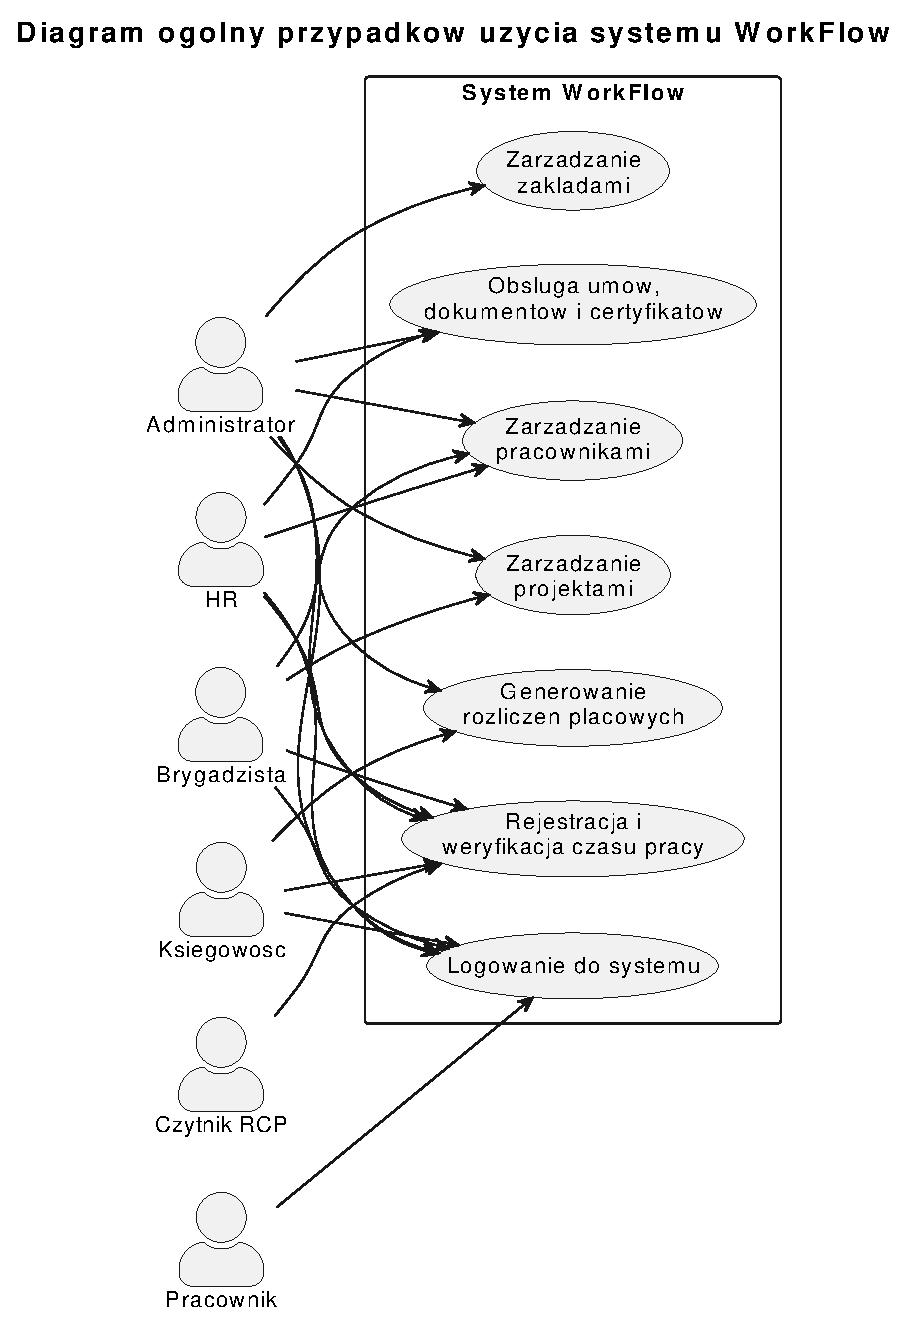
\includegraphics[width=\textwidth,height=0.82\textheight,keepaspectratio]{rys/plantuml-ogolny.pdf}
    \caption{Ogólny diagram przypadków użycia systemu \texttt{WorkFlow}}
    \label{fig:usecase-overall}
\end{figure}

\subsection{Modul kadrowy}

\begin{figure}[H]
    \centering
    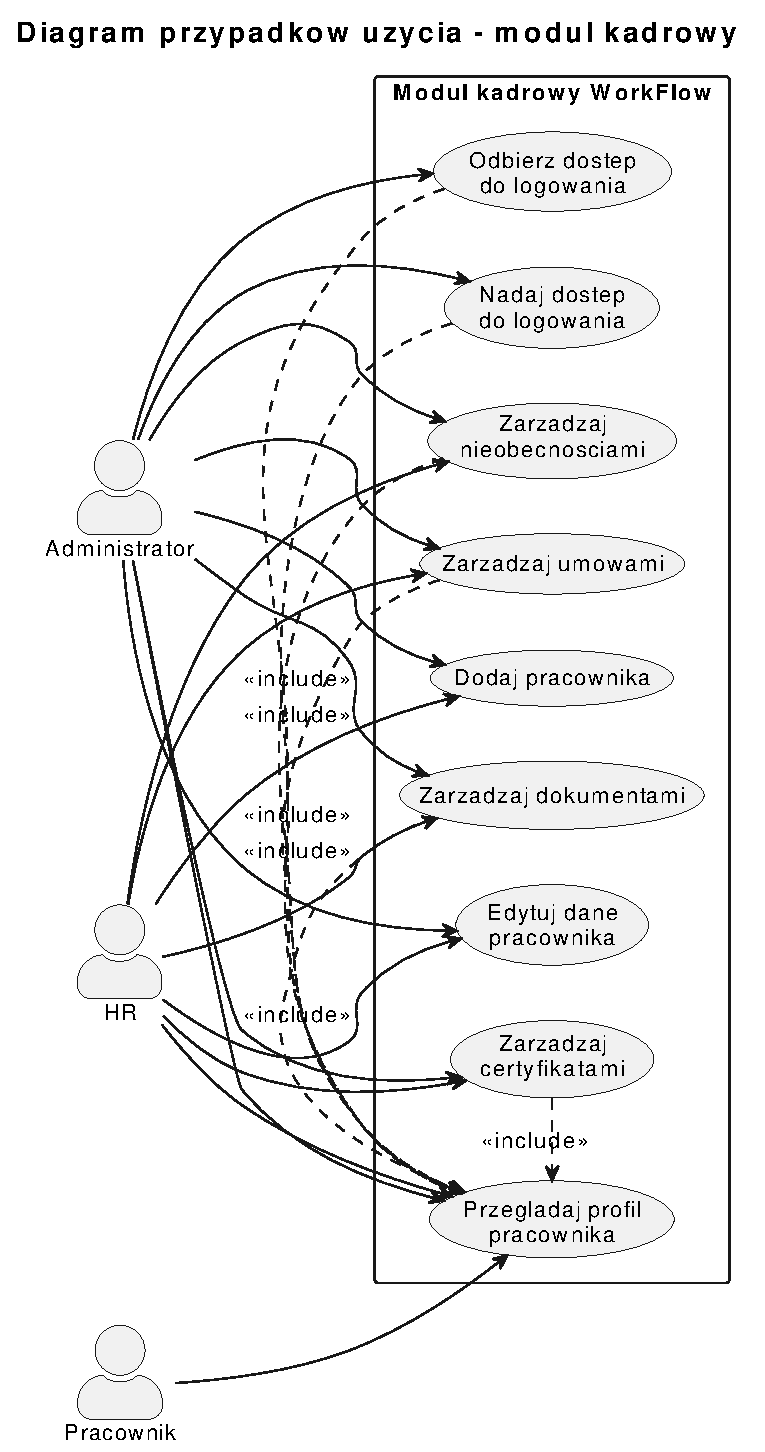
\includegraphics[width=\textwidth,height=0.82\textheight,keepaspectratio]{rys/plantuml-kadry.pdf}
    \caption{Diagram przypadków użycia dla modułu kadrowego}
    \label{fig:usecase-hr}
\end{figure}

\subsection{Czas pracy, RCP i rozliczenia}

\begin{figure}[H]
    \centering
    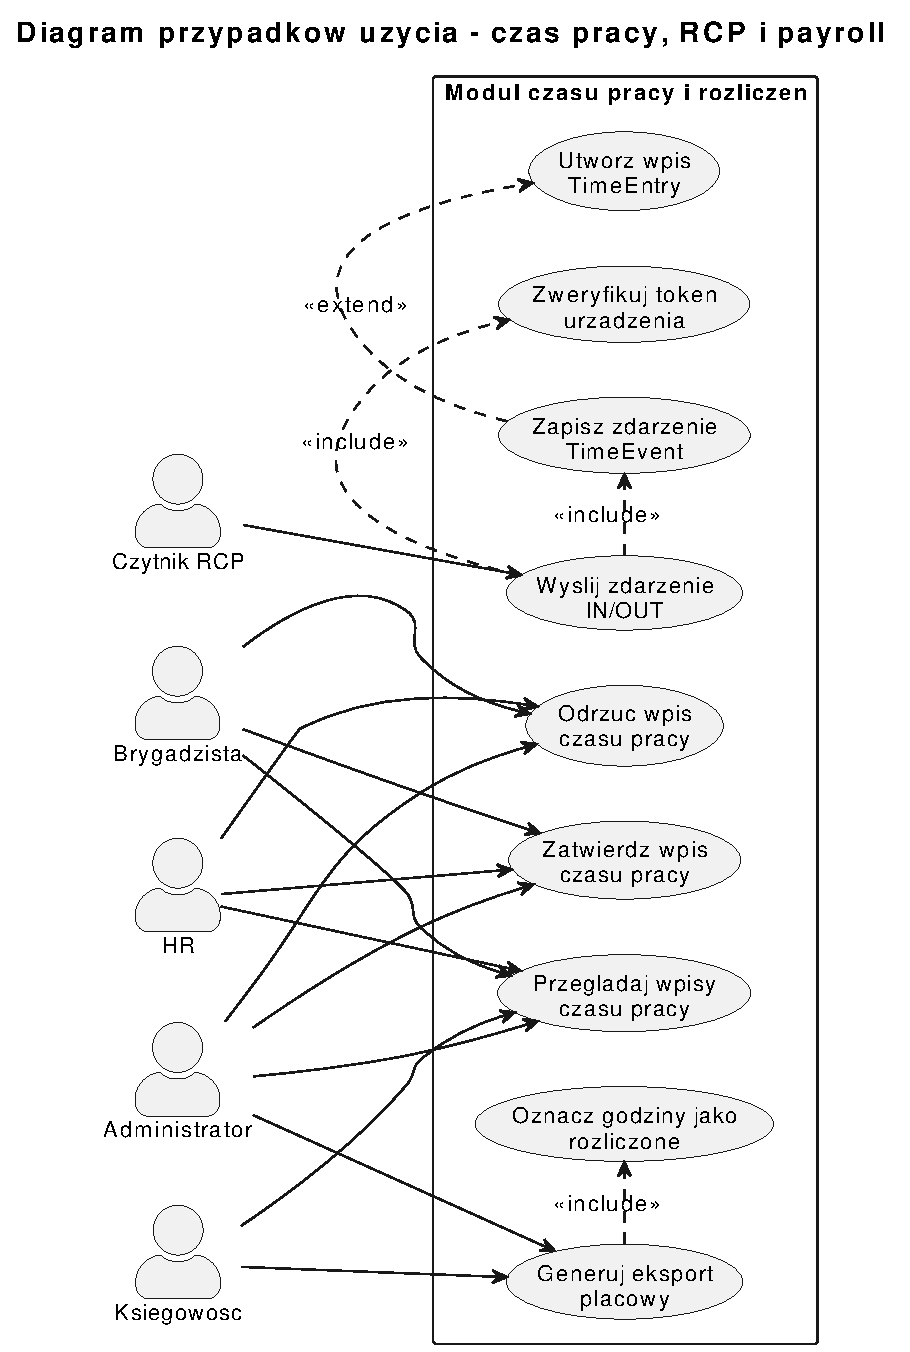
\includegraphics[width=\textwidth,height=0.82\textheight,keepaspectratio]{rys/plantuml-rcp-payroll.pdf}
    \caption{Diagram przypadków użycia dla rejestracji czasu pracy i rozliczeń}
    \label{fig:usecase-time}
\end{figure}

\subsection{Administracja i struktura organizacyjna}

\begin{figure}[H]
    \centering
    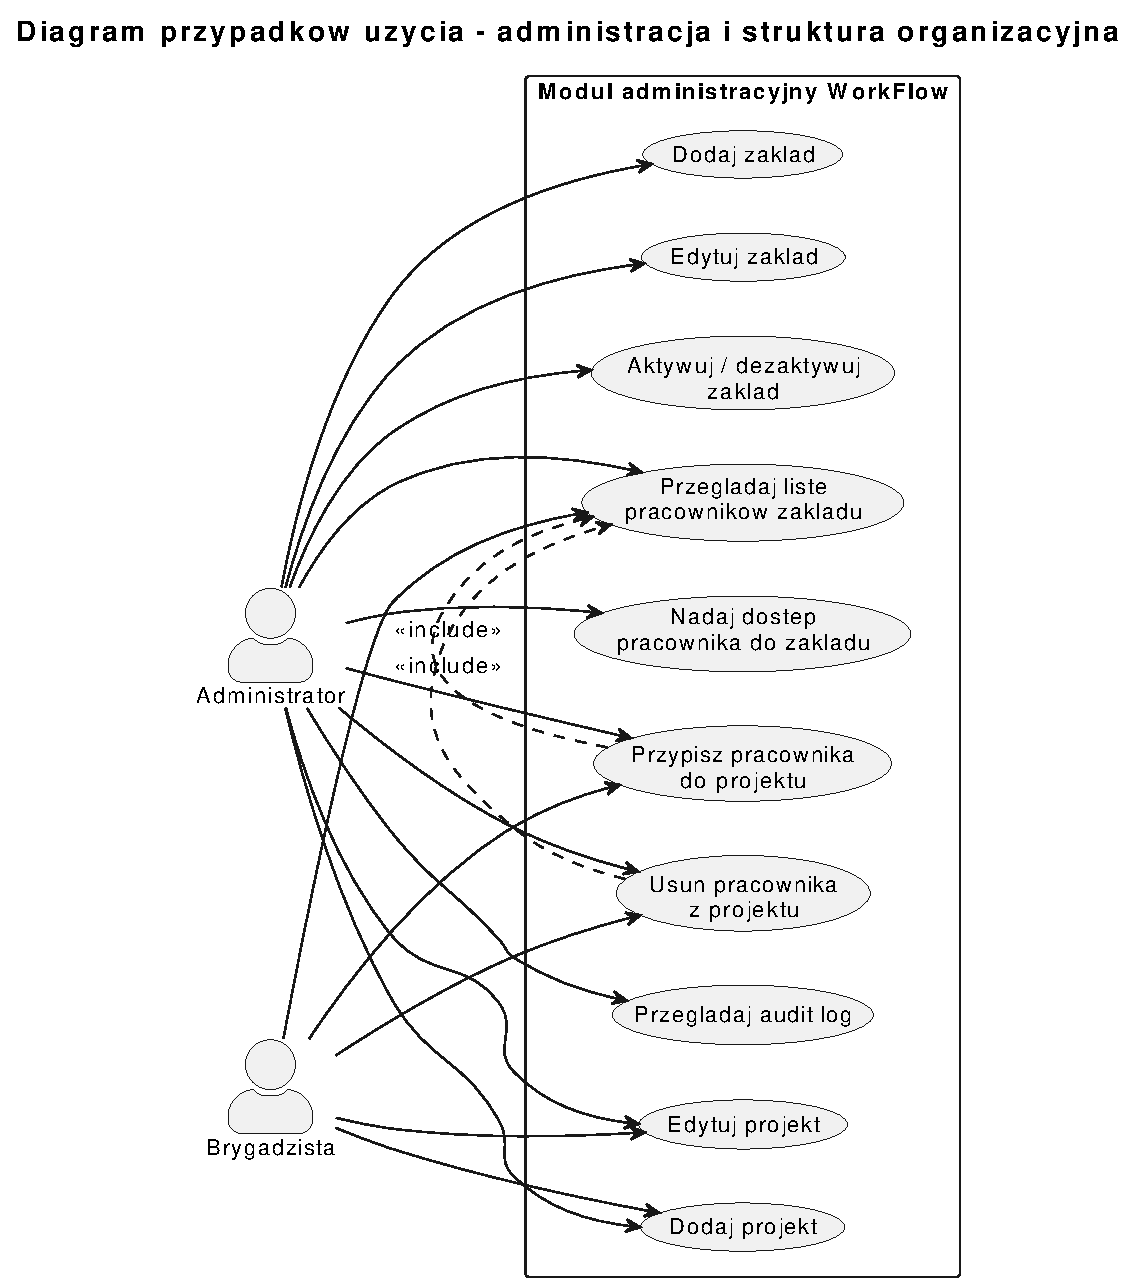
\includegraphics[width=\textwidth,height=0.82\textheight,keepaspectratio]{rys/plantuml-administracja.pdf}
    \caption{Diagram przypadków użycia dla administracji i zarządzania strukturą organizacyjną}
    \label{fig:usecase-admin}
\end{figure}

\subsection{Aktorzy systemu}

W systemie wyróżniono aktorów odpowiadających rolom użytkowników oraz jeden aktor techniczny reprezentujący czytnik RCP. Każdy aktor korzysta z innego zakresu funkcji, zgodnie z odpowiedzialnością w procesie obsługi pracowników, czasu pracy i dokumentacji.

\begin{itemize}
    \item \textbf{Administrator} -- użytkownik posiadający najszerszy zakres uprawnień. Odpowiada za ogólną konfigurację systemu, dostęp do zakładów, role użytkowników oraz kontrolę poprawności danych.
    \item \textbf{HR} -- użytkownik odpowiedzialny za obsługę danych kadrowych. Zarządza pracownikami, umowami, certyfikatami, dokumentami oraz nieobecnościami.
    \item \textbf{Księgowość} -- użytkownik korzystający z danych potrzebnych do rozliczeń. Pracuje głównie na zatwierdzonych wpisach czasu pracy i eksportach rozliczeniowych.
    \item \textbf{Brygadzista} -- użytkownik związany z pracą operacyjną. Ma dostęp do informacji dotyczących wybranych zakładów, projektów i pracowników.
    \item \textbf{Pracownik} -- podstawowa rola osoby znajdującej się w ewidencji systemu. W obecnym zakresie projektu rola ta pełni przede wszystkim funkcję danych pracowniczych, które są wykorzystywane przez inne moduły.
    \item \textbf{Czytnik RCP} -- aktor techniczny reprezentujący urządzenie wysyłające zdarzenia wejścia i wyjścia pracownika. Nie jest użytkownikiem interfejsu webowego, ale komunikuje się z backendem przez techniczny endpoint API.
\end{itemize}

\subsection{Zakres przypadków użycia}

Najważniejsze przypadki użycia systemu można podzielić na kilka grup funkcjonalnych:
\begin{itemize}
    \item \textbf{Uwierzytelnianie i dostęp} -- logowanie użytkownika, wylogowanie, sprawdzenie roli oraz zakresu dostępu do zakładów.
    \item \textbf{Zarządzanie strukturą organizacyjną} -- obsługa zakładów, przypisywanie pracowników do zakładów oraz nadawanie dostępu użytkownikom do wybranych jednostek.
    \item \textbf{Zarządzanie pracownikami} -- dodawanie, edycja, wyszukiwanie i przeglądanie pracowników oraz ich profili.
    \item \textbf{Zarządzanie projektami} -- tworzenie projektów, oznaczanie ich statusów oraz przypisywanie pracowników do projektów.
    \item \textbf{Rejestracja czasu pracy} -- odbieranie zdarzeń z czytników RCP, zapisywanie zdarzeń \texttt{IN}/\texttt{OUT} oraz tworzenie wpisów czasu pracy.
    \item \textbf{Obsługa dokumentacji kadrowej} -- obsługa umów, dokumentów, certyfikatów, badań, szkoleń i nieobecności.
    \item \textbf{Rozliczenia} -- przygotowanie danych rozliczeniowych oraz tworzenie eksportów payroll na podstawie zatwierdzonych wpisów czasu pracy.
    \item \textbf{Audyt} -- rejestrowanie wybranych operacji wykonywanych na danych systemu.
\end{itemize}

\subsection{Powiązanie ról z funkcjami}

Administrator posiada dostęp do największej liczby funkcji i odpowiada za konfigurację systemu oraz nadzór nad danymi. Rola HR koncentruje się na danych kadrowych, takich jak pracownicy, umowy, certyfikaty, nieobecności i dokumenty. Księgowość korzysta głównie z danych związanych z czasem pracy i rozliczeniami.

Brygadzista korzysta z danych operacyjnych, przede wszystkim z informacji o pracownikach, projektach i czasie pracy w ramach przypisanego obszaru. Pracownik jest podstawową encją systemu i może być powiązany z wieloma procesami, takimi jak przypisania do projektów, czas pracy, dokumenty, certyfikaty i nieobecności.

Czytnik RCP działa poza interfejsem użytkownika. Jego zadaniem jest przekazywanie zdarzeń technicznych do backendu. System na podstawie numeru seryjnego czytnika i identyfikatora karty RFID określa pracownika oraz projekt, którego dotyczy dane zdarzenie.

\subsection{Znaczenie diagramu dla projektu}

Diagram przypadków użycia porządkuje zakres funkcjonalny systemu i pokazuje, które role korzystają z poszczególnych modułów. Stanowi on punkt odniesienia dla dalszych scenariuszy użycia opisanych w kolejnym rozdziale.

Dzięki temu możliwe jest przejście od ogólnego obrazu funkcji systemu do konkretnych scenariuszy, takich jak logowanie użytkownika, zarządzanie profilem pracownika, rejestracja czasu pracy, kontrola ważności certyfikatów, obsługa nieobecności oraz przygotowanie danych rozliczeniowych.
% ================= SEKCJA 6 =================
\section{Scenariusze}

W niniejszym rozdziale przedstawiono scenariusze wybranych przypadków użycia systemu \texttt{WorkFlow}. Scenariusze opisują przebieg najważniejszych operacji z punktu widzenia użytkownika lub komponentu technicznego, a także wskazują warunki początkowe, przebieg podstawowy oraz możliwe warianty alternatywne.

Opisane scenariusze odpowiadają aktualnemu zakresowi projektu i obejmują logowanie, zarządzanie profilem pracownika, rejestrację czasu pracy z czytnika RCP, obsługę certyfikatów, nieobecności, umów, dokumentów oraz przygotowanie danych rozliczeniowych.

\subsection{SC-01: Logowanie użytkownika}
\begin{itemize}
    \item \textbf{Numer:} SC-01
    \item \textbf{Nazwa:} Logowanie użytkownika
    \item \textbf{Aktor:} Użytkownik systemu
    \item \textbf{Stan wejścia:}
    \begin{itemize}
        \item Użytkownik posiada konto w systemie.
        \item Konto ma przypisany adres e-mail, hash hasła oraz rolę systemową.
        \item Konto jest aktywne i ma włączoną możliwość logowania.
    \end{itemize}
    \item \textbf{Przebieg:}
    \begin{enumerate}
        \item Użytkownik otwiera formularz logowania.
        \item Wprowadza adres e-mail oraz hasło.
        \item System przesyła dane logowania do backendu.
        \item Backend wyszukuje użytkownika po adresie e-mail.
        \item Backend weryfikuje poprawność hasła.
        \item Po poprawnej weryfikacji system generuje token JWT.
        \item Token zostaje zapisany w ciasteczku sesyjnym.
        \item Użytkownik zostaje przekierowany do panelu aplikacji.
    \end{enumerate}
    \item \textbf{Zakończenie lub przebieg alternatywny:}
    \begin{itemize}
        \item \textbf{Zakończenie pozytywne:} Użytkownik zostaje zalogowany i uzyskuje dostęp do funkcji zgodnych ze swoją rolą.
        \item \textbf{Błędne dane logowania:} System odrzuca próbę logowania i wyświetla komunikat o błędnych poświadczeniach.
        \item \textbf{Konto nieaktywne lub bez dostępu do logowania:} System nie przyznaje dostępu do aplikacji.
    \end{itemize}
\end{itemize}

\subsection{SC-02: Zarządzanie profilem pracownika}
\begin{itemize}
    \item \textbf{Numer:} SC-02
    \item \textbf{Nazwa:} Zarządzanie profilem pracownika
    \item \textbf{Aktor:} HR lub Administrator
    \item \textbf{Stan wejścia:}
    \begin{itemize}
        \item Użytkownik jest zalogowany.
        \item Użytkownik posiada rolę umożliwiającą zarządzanie danymi pracowników.
        \item W systemie istnieje zakład, do którego można przypisać pracownika.
    \end{itemize}
    \item \textbf{Przebieg:}
    \begin{enumerate}
        \item Użytkownik przechodzi do listy pracowników.
        \item System wyświetla listę pracowników zgodną z zakresem dostępu użytkownika.
        \item Użytkownik wyszukuje pracownika lub otwiera formularz dodania nowej osoby.
        \item Użytkownik wprowadza albo modyfikuje dane podstawowe pracownika.
        \item Użytkownik określa zakład, rolę, status aktywności oraz opcjonalny identyfikator karty RFID.
        \item System waliduje poprawność danych, między innymi unikalność adresu e-mail, numeru PESEL i identyfikatora karty RFID.
        \item System zapisuje dane w bazie.
        \item Użytkownik może przejść do profilu pracownika i zarządzać powiązanymi informacjami.
    \end{enumerate}
    \item \textbf{Zakończenie lub przebieg alternatywny:}
    \begin{itemize}
        \item \textbf{Zakończenie pozytywne:} Dane pracownika zostają zapisane lub zaktualizowane.
        \item \textbf{Błąd walidacji:} System wyświetla komunikat i wskazuje pola wymagające poprawy.
        \item \textbf{Brak uprawnień:} System blokuje operację, jeżeli użytkownik nie posiada odpowiedniej roli lub dostępu do zakładu.
    \end{itemize}
\end{itemize}

\subsection{SC-03: Rejestracja czasu pracy przez czytnik RCP}
\begin{itemize}
    \item \textbf{Numer:} SC-03
    \item \textbf{Nazwa:} Rejestracja czasu pracy przez czytnik RCP
    \item \textbf{Aktor:} Czytnik RCP
    \item \textbf{Stan wejścia:}
    \begin{itemize}
        \item W systemie istnieje aktywny czytnik RCP.
        \item Czytnik jest przypisany do zakładu i projektu.
        \item Pracownik posiada przypisany identyfikator karty RFID.
        \item Endpoint urządzenia jest zabezpieczony tokenem technicznym.
    \end{itemize}
    \item \textbf{Przebieg:}
    \begin{enumerate}
        \item Pracownik odbija kartę RFID na czytniku.
        \item Czytnik wysyła do backendu zdarzenie zawierające numer seryjny czytnika, identyfikator karty, typ zdarzenia oraz czas zdarzenia.
        \item Backend weryfikuje token urządzenia.
        \item System wyszukuje aktywny czytnik na podstawie numeru seryjnego.
        \item System wyszukuje aktywnego pracownika na podstawie identyfikatora karty RFID.
        \item System sprawdza, czy pracownik ma dostęp do zakładu powiązanego z czytnikiem.
        \item System zapisuje surowe zdarzenie w tabeli \texttt{TimeEvent}.
        \item Jeżeli zdarzenie ma typ \texttt{OUT}, system wyszukuje wcześniejsze zdarzenie \texttt{IN}.
        \item Na podstawie pary zdarzeń \texttt{IN}/\texttt{OUT} system tworzy wpis czasu pracy w tabeli \texttt{TimeEntry}.
    \end{enumerate}
    \item \textbf{Zakończenie lub przebieg alternatywny:}
    \begin{itemize}
        \item \textbf{Zakończenie pozytywne:} Zdarzenie zostaje zapisane, a dla zdarzenia \texttt{OUT} powstaje wpis czasu pracy.
        \item \textbf{Nieznany czytnik:} System odrzuca zdarzenie, jeżeli numer seryjny nie odpowiada aktywnemu czytnikowi.
        \item \textbf{Nieznana karta RFID:} System odrzuca zdarzenie, jeżeli nie znajdzie aktywnego pracownika.
        \item \textbf{Brak wcześniejszego wejścia:} System zapisuje błąd logiczny i nie tworzy wpisu czasu pracy dla zdarzenia \texttt{OUT}.
    \end{itemize}
\end{itemize}

\subsection{SC-04: Weryfikacja wpisów czasu pracy}
\begin{itemize}
    \item \textbf{Numer:} SC-04
    \item \textbf{Nazwa:} Weryfikacja wpisów czasu pracy
    \item \textbf{Aktor:} HR, Administrator lub użytkownik uprawniony do weryfikacji
    \item \textbf{Stan wejścia:}
    \begin{itemize}
        \item W systemie istnieją wpisy czasu pracy.
        \item Wpisy posiadają status, na przykład \texttt{PENDING}.
        \item Użytkownik posiada uprawnienia do przeglądania i weryfikowania wpisów czasu pracy.
    \end{itemize}
    \item \textbf{Przebieg:}
    \begin{enumerate}
        \item Użytkownik przechodzi do widoku czasu pracy.
        \item System wyświetla wpisy czasu pracy z wybranego zakresu.
        \item Użytkownik analizuje dane pracownika, projekt, czas rozpoczęcia, czas zakończenia oraz liczbę godzin.
        \item Użytkownik zatwierdza poprawny wpis albo oznacza go jako wymagający odrzucenia.
        \item System aktualizuje status wpisu czasu pracy.
        \item Zatwierdzone wpisy mogą zostać wykorzystane w module rozliczeń.
    \end{enumerate}
    \item \textbf{Zakończenie lub przebieg alternatywny:}
    \begin{itemize}
        \item \textbf{Zakończenie pozytywne:} Wpis uzyskuje status \texttt{APPROVED} i może zostać uwzględniony w rozliczeniach.
        \item \textbf{Odrzucenie wpisu:} Wpis uzyskuje status \texttt{REJECTED} i nie jest brany pod uwagę przy eksporcie payroll.
        \item \textbf{Brak uprawnień:} System blokuje zmianę statusu wpisu.
    \end{itemize}
\end{itemize}

\subsection{SC-05: Dodanie umowy pracownika}
\begin{itemize}
    \item \textbf{Numer:} SC-05
    \item \textbf{Nazwa:} Dodanie umowy pracownika
    \item \textbf{Aktor:} HR lub Administrator
    \item \textbf{Stan wejścia:}
    \begin{itemize}
        \item Użytkownik jest zalogowany.
        \item Użytkownik posiada dostęp do profilu pracownika.
        \item Pracownik istnieje w systemie.
    \end{itemize}
    \item \textbf{Przebieg:}
    \begin{enumerate}
        \item Użytkownik otwiera profil pracownika.
        \item Przechodzi do sekcji umów.
        \item Wybiera opcję dodania nowej umowy.
        \item Wprowadza typ umowy, kwotę wynagrodzenia, datę rozpoczęcia oraz opcjonalną datę zakończenia.
        \item Określa, czy umowa jest aktualna.
        \item System waliduje dane formularza.
        \item System zapisuje umowę i przypisuje ją do pracownika.
    \end{enumerate}
    \item \textbf{Zakończenie lub przebieg alternatywny:}
    \begin{itemize}
        \item \textbf{Zakończenie pozytywne:} Umowa zostaje zapisana w historii umów pracownika.
        \item \textbf{Brak wymaganych danych:} System wyświetla komunikat i nie zapisuje umowy.
        \item \textbf{Brak uprawnień:} System blokuje operację.
    \end{itemize}
\end{itemize}

\subsection{SC-06: Monitorowanie ważności certyfikatów}
\begin{itemize}
    \item \textbf{Numer:} SC-06
    \item \textbf{Nazwa:} Monitorowanie ważności certyfikatów
    \item \textbf{Aktor:} HR lub Administrator
    \item \textbf{Stan wejścia:}
    \begin{itemize}
        \item W systemie istnieje słownik certyfikatów.
        \item Pracownicy posiadają przypisane certyfikaty z datą wydania i datą ważności.
        \item Użytkownik posiada dostęp do modułu certyfikatów.
    \end{itemize}
    \item \textbf{Przebieg:}
    \begin{enumerate}
        \item Użytkownik przechodzi do widoku certyfikatów wygasających.
        \item Wybiera zakres czasu, na przykład 30, 90 lub 365 dni.
        \item System pobiera certyfikaty, których data ważności mieści się w wybranym zakresie.
        \item System prezentuje dane pracownika, typ certyfikatu, nazwę dokumentu oraz liczbę dni do wygaśnięcia.
        \item Użytkownik może przejść do profilu pracownika i uzupełnić lub zaktualizować dane certyfikatu.
    \end{enumerate}
    \item \textbf{Zakończenie lub przebieg alternatywny:}
    \begin{itemize}
        \item \textbf{Zakończenie pozytywne:} Użytkownik otrzymuje listę certyfikatów wymagających kontroli.
        \item \textbf{Brak wyników:} System wyświetla pustą listę dla wybranego zakresu.
        \item \textbf{Brak dostępu do zakładu:} System nie pokazuje danych spoza zakresu uprawnień użytkownika.
    \end{itemize}
\end{itemize}

\subsection{SC-07: Dodanie nieobecności pracownika}
\begin{itemize}
    \item \textbf{Numer:} SC-07
    \item \textbf{Nazwa:} Dodanie nieobecności pracownika
    \item \textbf{Aktor:} HR lub Administrator
    \item \textbf{Stan wejścia:}
    \begin{itemize}
        \item Użytkownik jest zalogowany.
        \item Pracownik istnieje w systemie.
        \item Użytkownik posiada dostęp do profilu pracownika.
    \end{itemize}
    \item \textbf{Przebieg:}
    \begin{enumerate}
        \item Użytkownik otwiera profil pracownika.
        \item Przechodzi do sekcji nieobecności.
        \item Wybiera opcję dodania nowej nieobecności.
        \item Określa typ nieobecności, datę rozpoczęcia i datę zakończenia.
        \item Opcjonalnie wskazuje dokument powiązany z nieobecnością.
        \item Określa, czy nieobecność jest zatwierdzona.
        \item System zapisuje nieobecność i przypisuje ją do pracownika.
    \end{enumerate}
    \item \textbf{Zakończenie lub przebieg alternatywny:}
    \begin{itemize}
        \item \textbf{Zakończenie pozytywne:} Nieobecność pojawia się w profilu pracownika.
        \item \textbf{Niepoprawny zakres dat:} System odrzuca zapis i wyświetla komunikat.
        \item \textbf{Brak uprawnień:} System blokuje operację.
    \end{itemize}
\end{itemize}

\subsection{SC-08: Dodanie dokumentu pracownika}
\begin{itemize}
    \item \textbf{Numer:} SC-08
    \item \textbf{Nazwa:} Dodanie dokumentu pracownika
    \item \textbf{Aktor:} HR lub Administrator
    \item \textbf{Stan wejścia:}
    \begin{itemize}
        \item Użytkownik posiada dostęp do profilu pracownika.
        \item Pracownik istnieje w systemie.
        \item Magazyn plików jest skonfigurowany.
    \end{itemize}
    \item \textbf{Przebieg:}
    \begin{enumerate}
        \item Użytkownik otwiera profil pracownika.
        \item Wybiera opcję dodania dokumentu.
        \item Wskazuje plik dokumentu lub dane dokumentu.
        \item System zapisuje plik w magazynie obiektowym albo zapisuje jego ścieżkę.
        \item System tworzy rekord dokumentu w bazie danych.
        \item Dokument zostaje powiązany z pracownikiem oraz opcjonalnie z umową lub certyfikatem.
    \end{enumerate}
    \item \textbf{Zakończenie lub przebieg alternatywny:}
    \begin{itemize}
        \item \textbf{Zakończenie pozytywne:} Dokument zostaje zapisany i widoczny w danych pracownika.
        \item \textbf{Błąd zapisu pliku:} System informuje użytkownika o problemie z magazynem plików.
        \item \textbf{Brak danych wymaganych:} System nie tworzy rekordu dokumentu.
    \end{itemize}
\end{itemize}

\subsection{SC-09: Przygotowanie eksportu rozliczeniowego}
\begin{itemize}
    \item \textbf{Numer:} SC-09
    \item \textbf{Nazwa:} Przygotowanie eksportu rozliczeniowego
    \item \textbf{Aktor:} Księgowość
    \item \textbf{Stan wejścia:}
    \begin{itemize}
        \item Użytkownik jest zalogowany i posiada rolę księgowości.
        \item W systemie istnieją zatwierdzone wpisy czasu pracy.
        \item Wpisy nie zostały wcześniej powiązane z eksportem payroll.
    \end{itemize}
    \item \textbf{Przebieg:}
    \begin{enumerate}
        \item Użytkownik przechodzi do modułu rozliczeń.
        \item Wybiera miesiąc i rok rozliczeniowy.
        \item System pobiera zatwierdzone wpisy czasu pracy z wybranego okresu.
        \item System tworzy rekord eksportu rozliczeniowego.
        \item System zapisuje liczbę pracowników objętych eksportem.
        \item System wiąże wybrane wpisy czasu pracy z eksportem.
        \item Użytkownik otrzymuje informację o przygotowaniu danych.
    \end{enumerate}
    \item \textbf{Zakończenie lub przebieg alternatywny:}
    \begin{itemize}
        \item \textbf{Zakończenie pozytywne:} Eksport zostaje utworzony, a powiązane wpisy czasu pracy są oznaczone jako rozliczone w ramach danej paczki.
        \item \textbf{Brak zatwierdzonych wpisów:} System nie tworzy eksportu i informuje użytkownika o braku danych.
        \item \textbf{Dane już wyeksportowane:} System pomija wpisy powiązane z wcześniejszym eksportem.
    \end{itemize}
\end{itemize}

\subsection{SC-10: Uruchomienie danych demonstracyjnych}
\begin{itemize}
    \item \textbf{Numer:} SC-10
    \item \textbf{Nazwa:} Uruchomienie danych demonstracyjnych
    \item \textbf{Aktor:} Administrator techniczny
    \item \textbf{Stan wejścia:}
    \begin{itemize}
        \item Środowisko Docker Compose jest uruchomione.
        \item Backend ma dostęp do bazy danych.
        \item W środowisku ustawiono zmienną potwierdzającą zgodę na wykonanie seeda demonstracyjnego.
    \end{itemize}
    \item \textbf{Przebieg:}
    \begin{enumerate}
        \item Administrator techniczny uruchamia komendę seeda demonstracyjnego.
        \item Skrypt sprawdza obecność wymaganej zmiennej środowiskowej.
        \item Skrypt czyści dane przeznaczone do prezentacji.
        \item Skrypt tworzy zakłady, użytkowników, pracowników, projekty, czytniki RCP, umowy, certyfikaty, dokumenty, nieobecności, zdarzenia czasu pracy i eksport rozliczeniowy.
        \item Administrator loguje się do aplikacji na konto testowe.
        \item System prezentuje komplet przykładowych danych.
    \end{enumerate}
    \item \textbf{Zakończenie lub przebieg alternatywny:}
    \begin{itemize}
        \item \textbf{Zakończenie pozytywne:} Baza danych zawiera komplet danych demonstracyjnych gotowych do prezentacji projektu.
        \item \textbf{Brak zmiennej zabezpieczającej:} Skrypt przerywa działanie i nie modyfikuje bazy.
        \item \textbf{Błąd połączenia z bazą:} Skrypt kończy się błędem i wyświetla komunikat diagnostyczny.
    \end{itemize}
\end{itemize}
% ================= SEKCJA 7 =================
\section{Makiety i interfejs użytkownika}

Interfejs użytkownika systemu \texttt{WorkFlow} został zaprojektowany z myślą o pracy administracyjnej wykonywanej z poziomu przeglądarki internetowej. Głównym założeniem było przygotowanie widoków, które pozwalają szybko przejść do najważniejszych modułów systemu: pracowników, zakładów, projektów, czasu pracy, certyfikatów, dokumentów, nieobecności oraz rozliczeń.

W początkowej fazie projektu przygotowano makiety interfejsu, które pozwoliły określić ogólny układ aplikacji oraz rozmieszczenie najważniejszych informacji. W późniejszej implementacji część widoków została dostosowana do aktualnego zakresu funkcjonalnego systemu oraz do zastosowanego stosu technologicznego.

\subsection{Założenia projektowe interfejsu}

Podczas projektowania interfejsu przyjęto następujące założenia:
\begin{itemize}
    \item system powinien posiadać czytelną nawigację boczną,
    \item główne moduły powinny być dostępne z poziomu panelu użytkownika,
    \item widoki powinny być spójne pod względem układu formularzy, tabel i przycisków,
    \item dane powinny być możliwe do filtrowania i wyszukiwania,
    \item formularze powinny wskazywać wymagane dane oraz obsługiwać błędy walidacji,
    \item interfejs powinien poprawnie działać w trybie jasnym i ciemnym,
    \item użytkownik powinien widzieć tylko te elementy, do których ma dostęp zgodnie ze swoją rolą.
\end{itemize}

Aplikacja ma charakter panelu administracyjnego. Z tego względu najważniejsza była czytelność danych, łatwość przeglądania tabel oraz możliwość szybkiego przejścia do szczegółów rekordu.

\subsection{Pulpit główny}

Pulpit główny stanowi pierwszy ekran po zalogowaniu użytkownika. Jego zadaniem jest zebranie najważniejszych informacji oraz zapewnienie szybkiego dostępu do modułów systemu.

\begin{figure}[H]
    \centering
    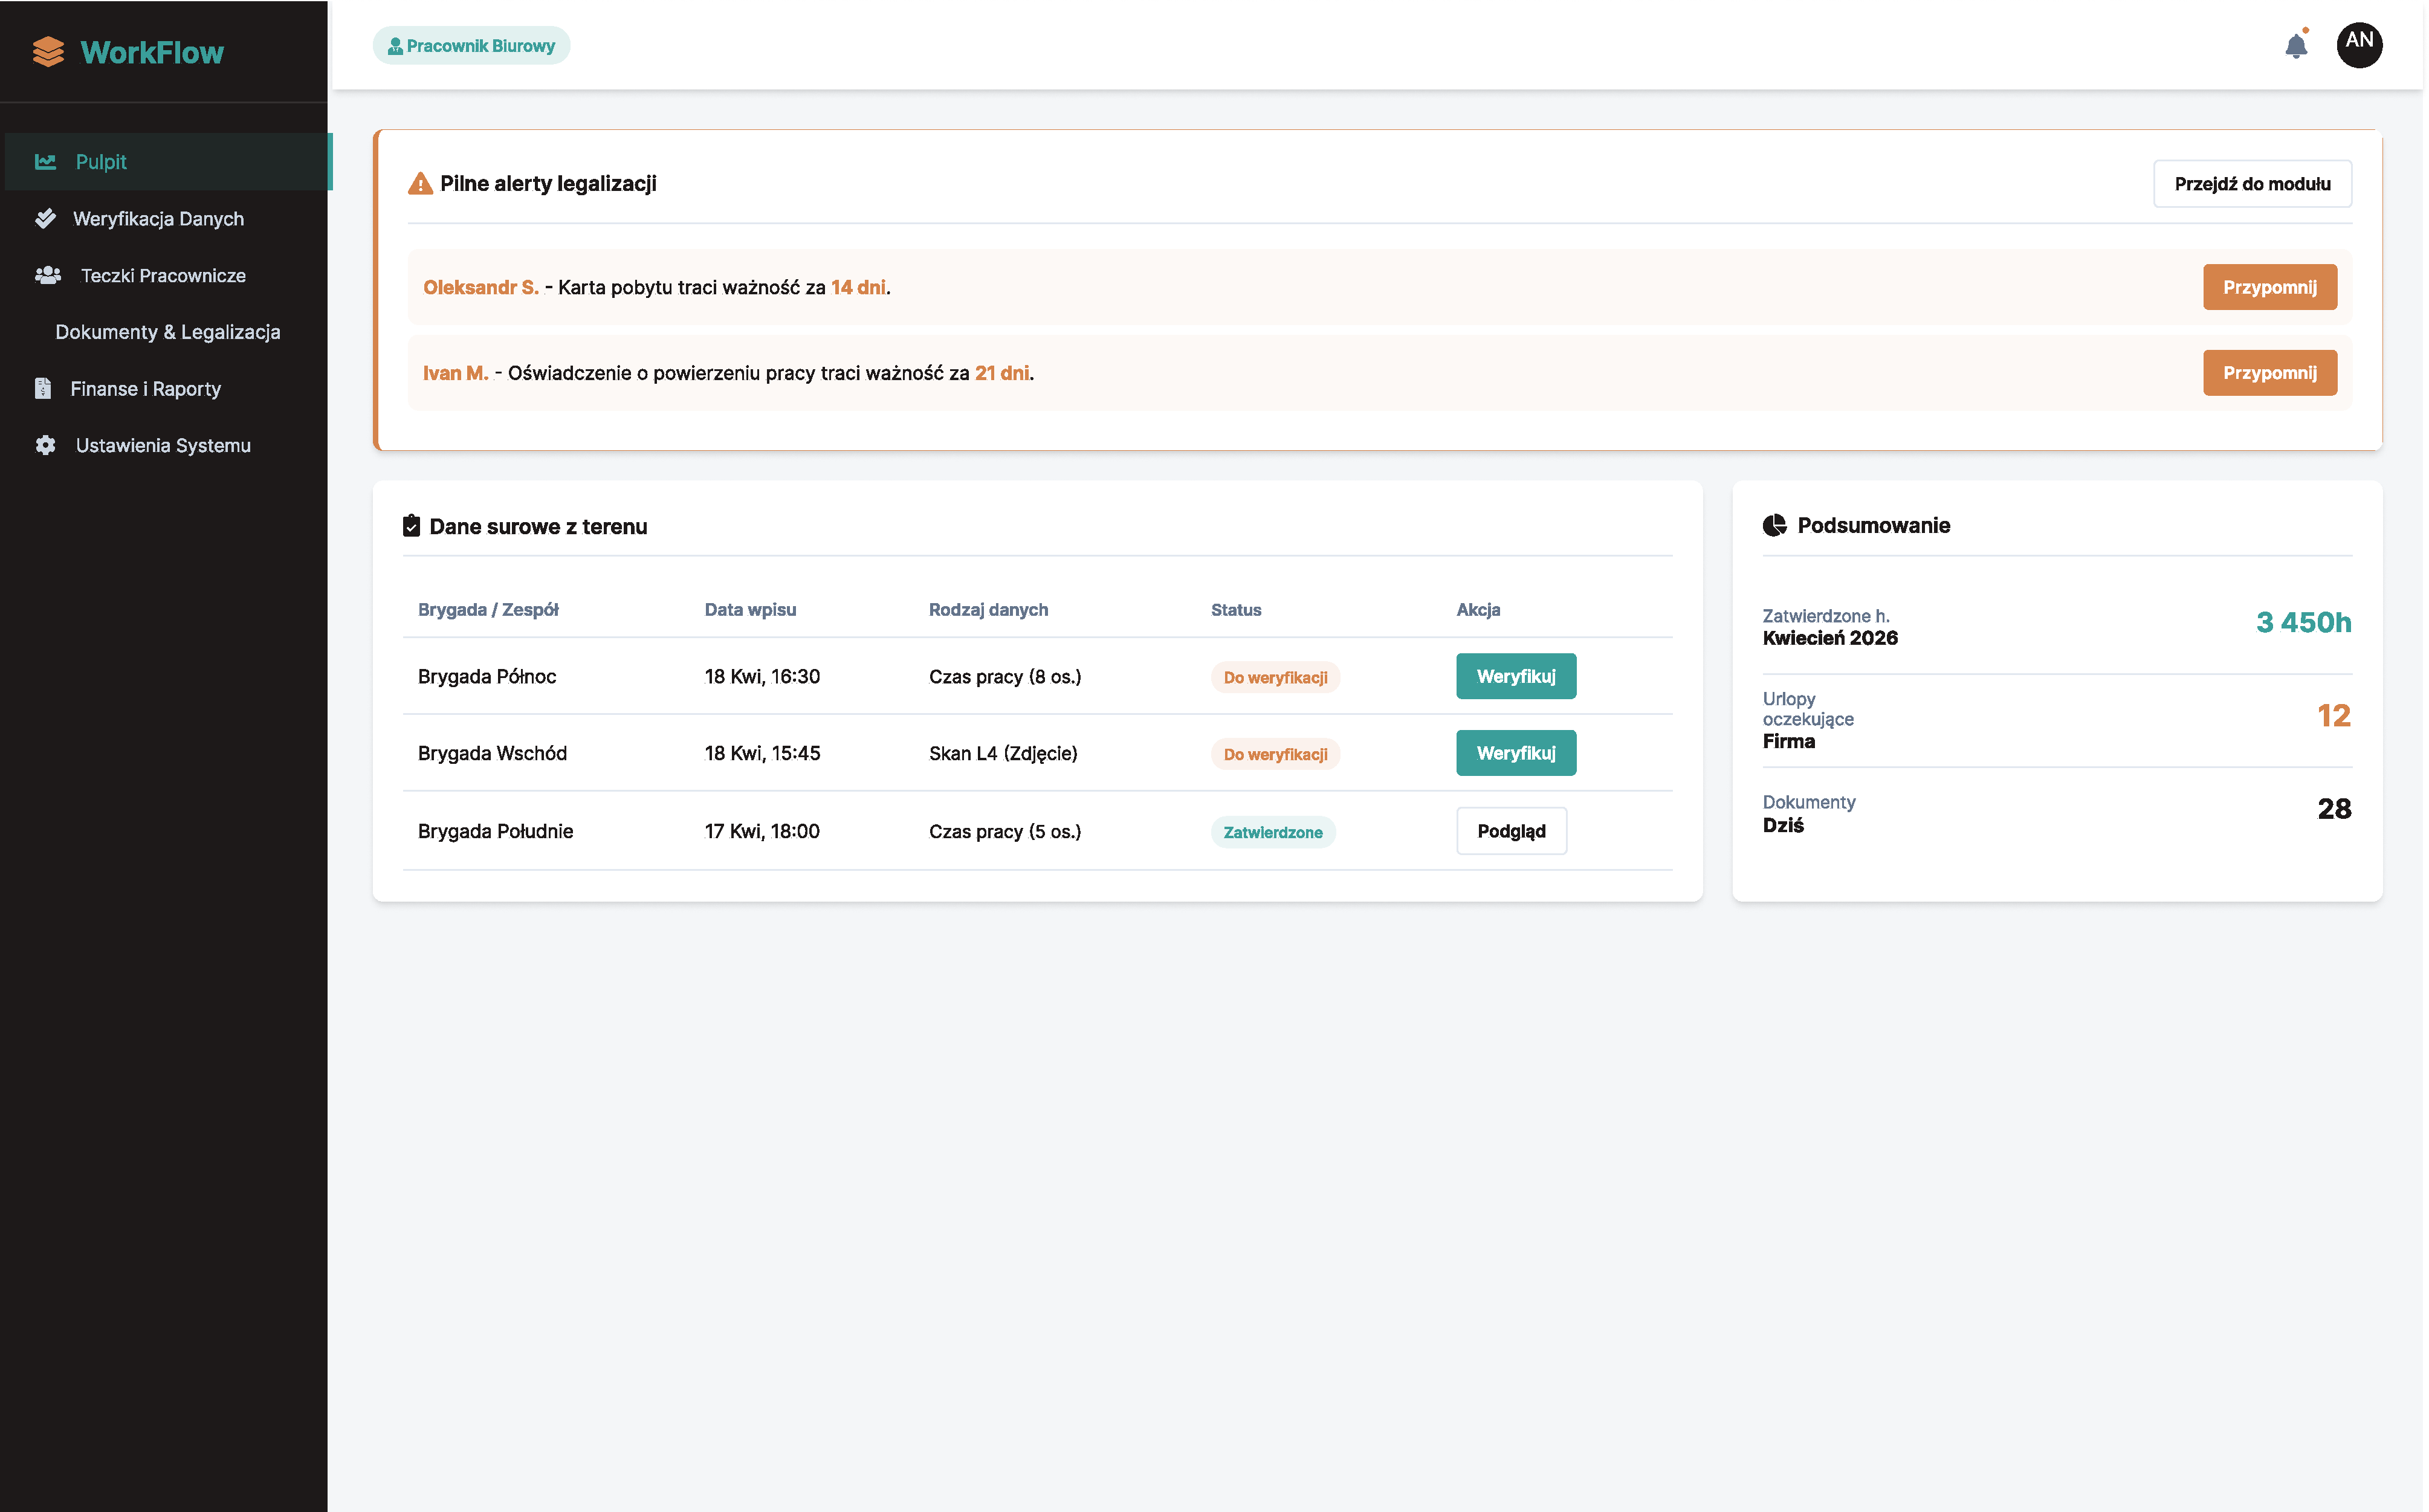
\includegraphics[width=0.95\textwidth]{rys/1920w.pdf}
    \caption{Widok desktopowy -- pulpit główny systemu \texttt{WorkFlow}}
    \label{fig:figma_dashboard_desktop}
\end{figure}

\begin{figure}[H]
    \centering
    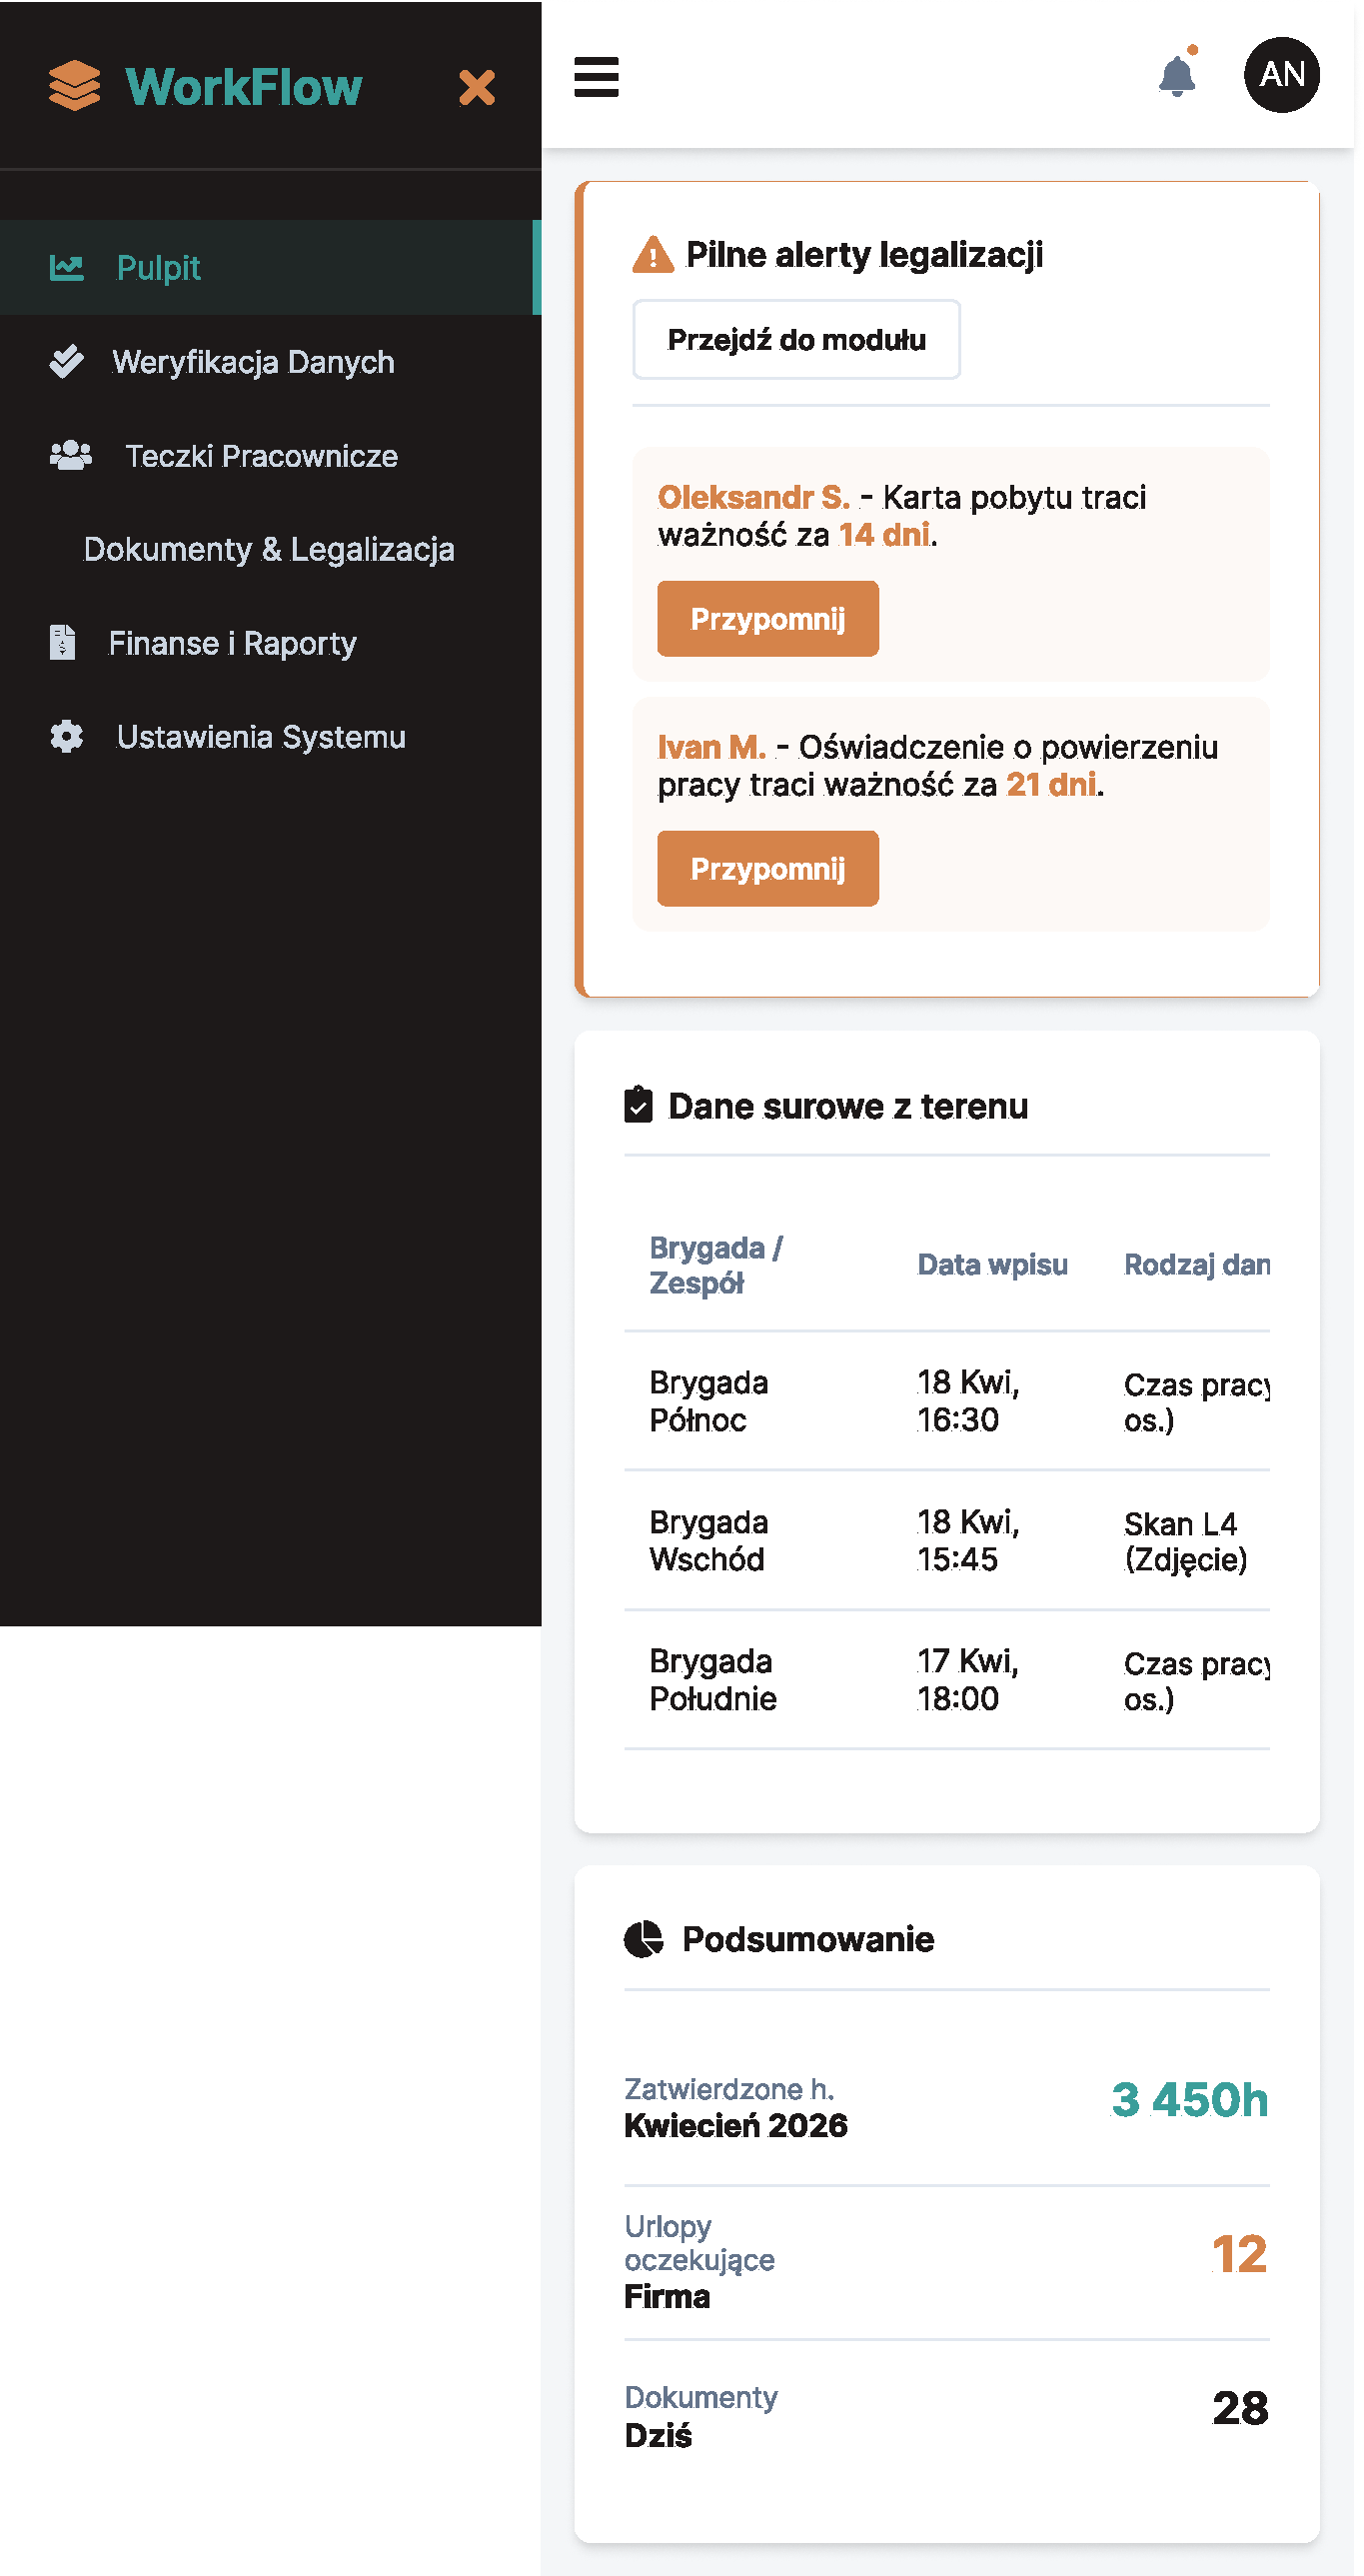
\includegraphics[width=0.35\textwidth]{rys/390w.pdf}
    \caption{Widok mobilny -- pulpit główny systemu \texttt{WorkFlow}}
    \label{fig:figma_dashboard_mobile}
\end{figure}

\textbf{Najważniejsze elementy pulpitu:}
\begin{itemize}
    \item \textbf{Nawigacja do modułów} -- użytkownik może przejść do widoków pracowników, zakładów, projektów, czasu pracy, certyfikatów i rozliczeń.
    \item \textbf{Kontekst zakładu} -- system uwzględnia zakład aktywny dla użytkownika, co pozwala ograniczyć zakres prezentowanych danych.
    \item \textbf{Podsumowania} -- widok może prezentować skrócone informacje dotyczące pracowników, projektów, certyfikatów lub czasu pracy.
    \item \textbf{Dostęp zależny od roli} -- zakres widocznych elementów zależy od tego, czy użytkownik pełni rolę administratora, HR, księgowości, brygadzisty lub inną rolę systemową.
\end{itemize}

Pulpit główny nie jest samodzielnym modułem biznesowym. Pełni rolę punktu startowego, który pozwala użytkownikowi przejść do dalszych obszarów systemu.

\subsection{Profil pracownika}

Profil pracownika jest jednym z najważniejszych widoków systemu. Łączy w jednym miejscu dane podstawowe pracownika oraz informacje powiązane z innymi modułami.

\begin{figure}[H]
    \centering
    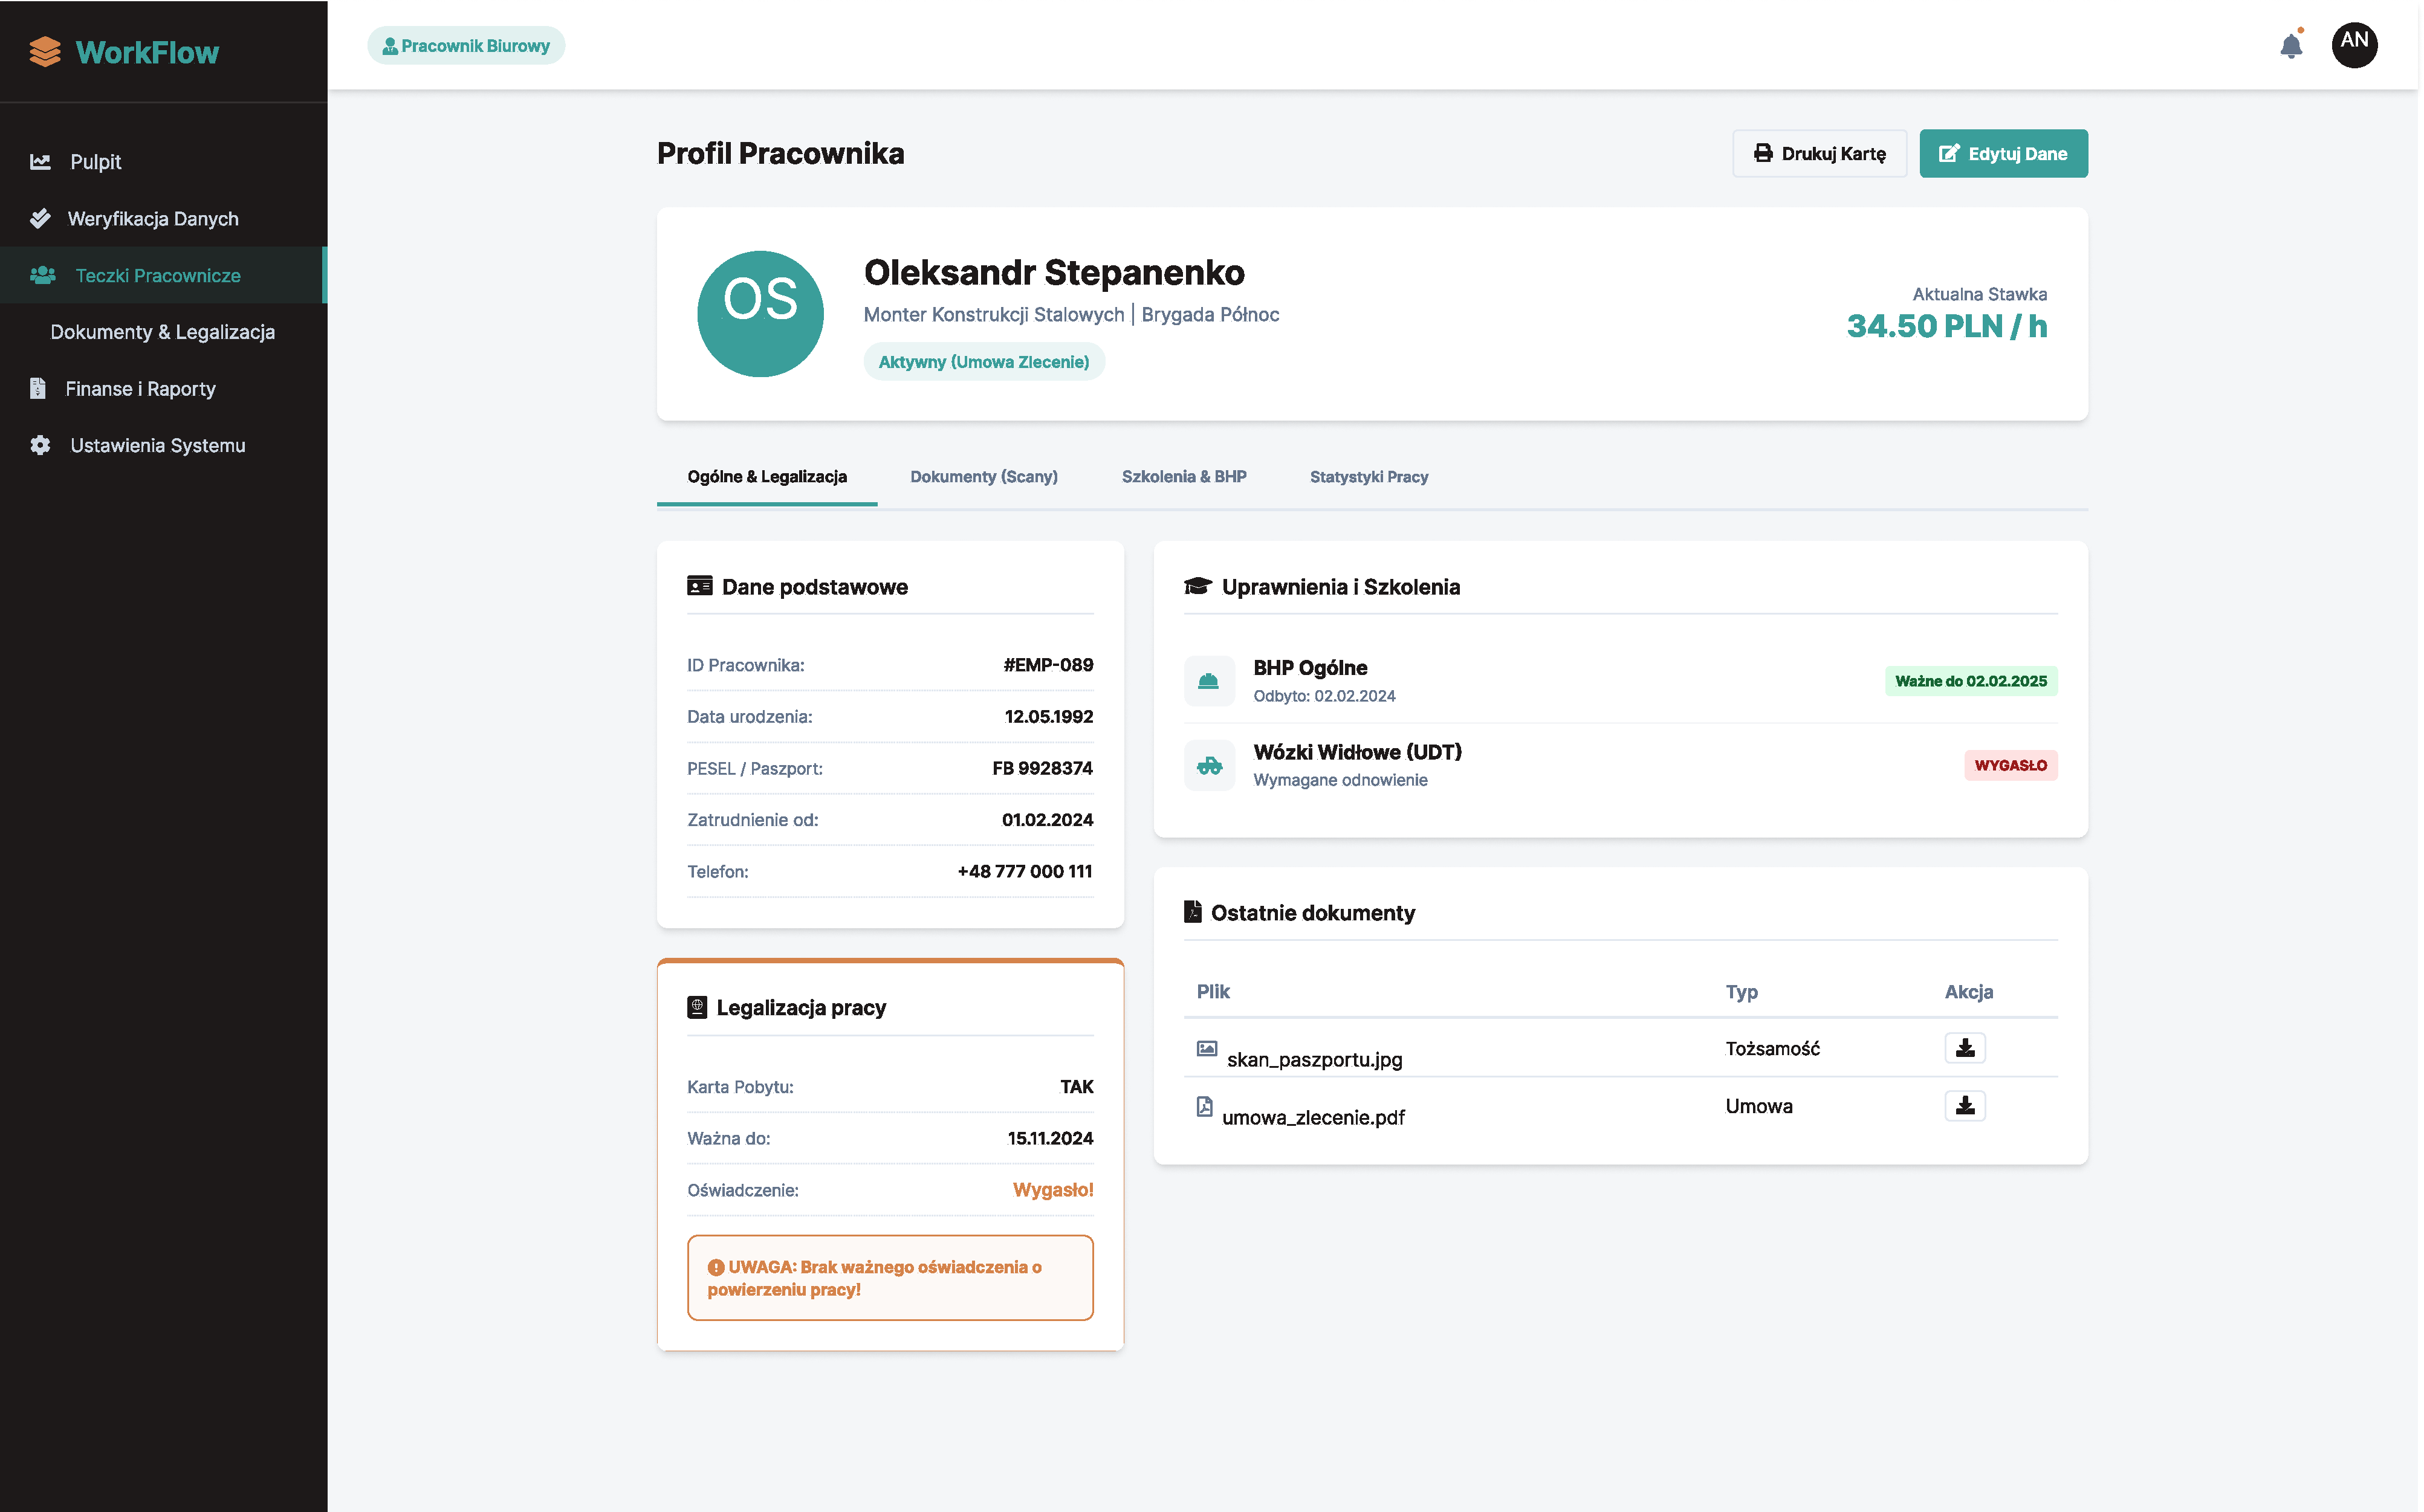
\includegraphics[width=0.95\textwidth]{rys/1920w_panel.pdf}
    \caption{Widok desktopowy -- profil pracownika}
    \label{fig:figma_profile_desktop}
\end{figure}

\begin{figure}[H]
    \centering
    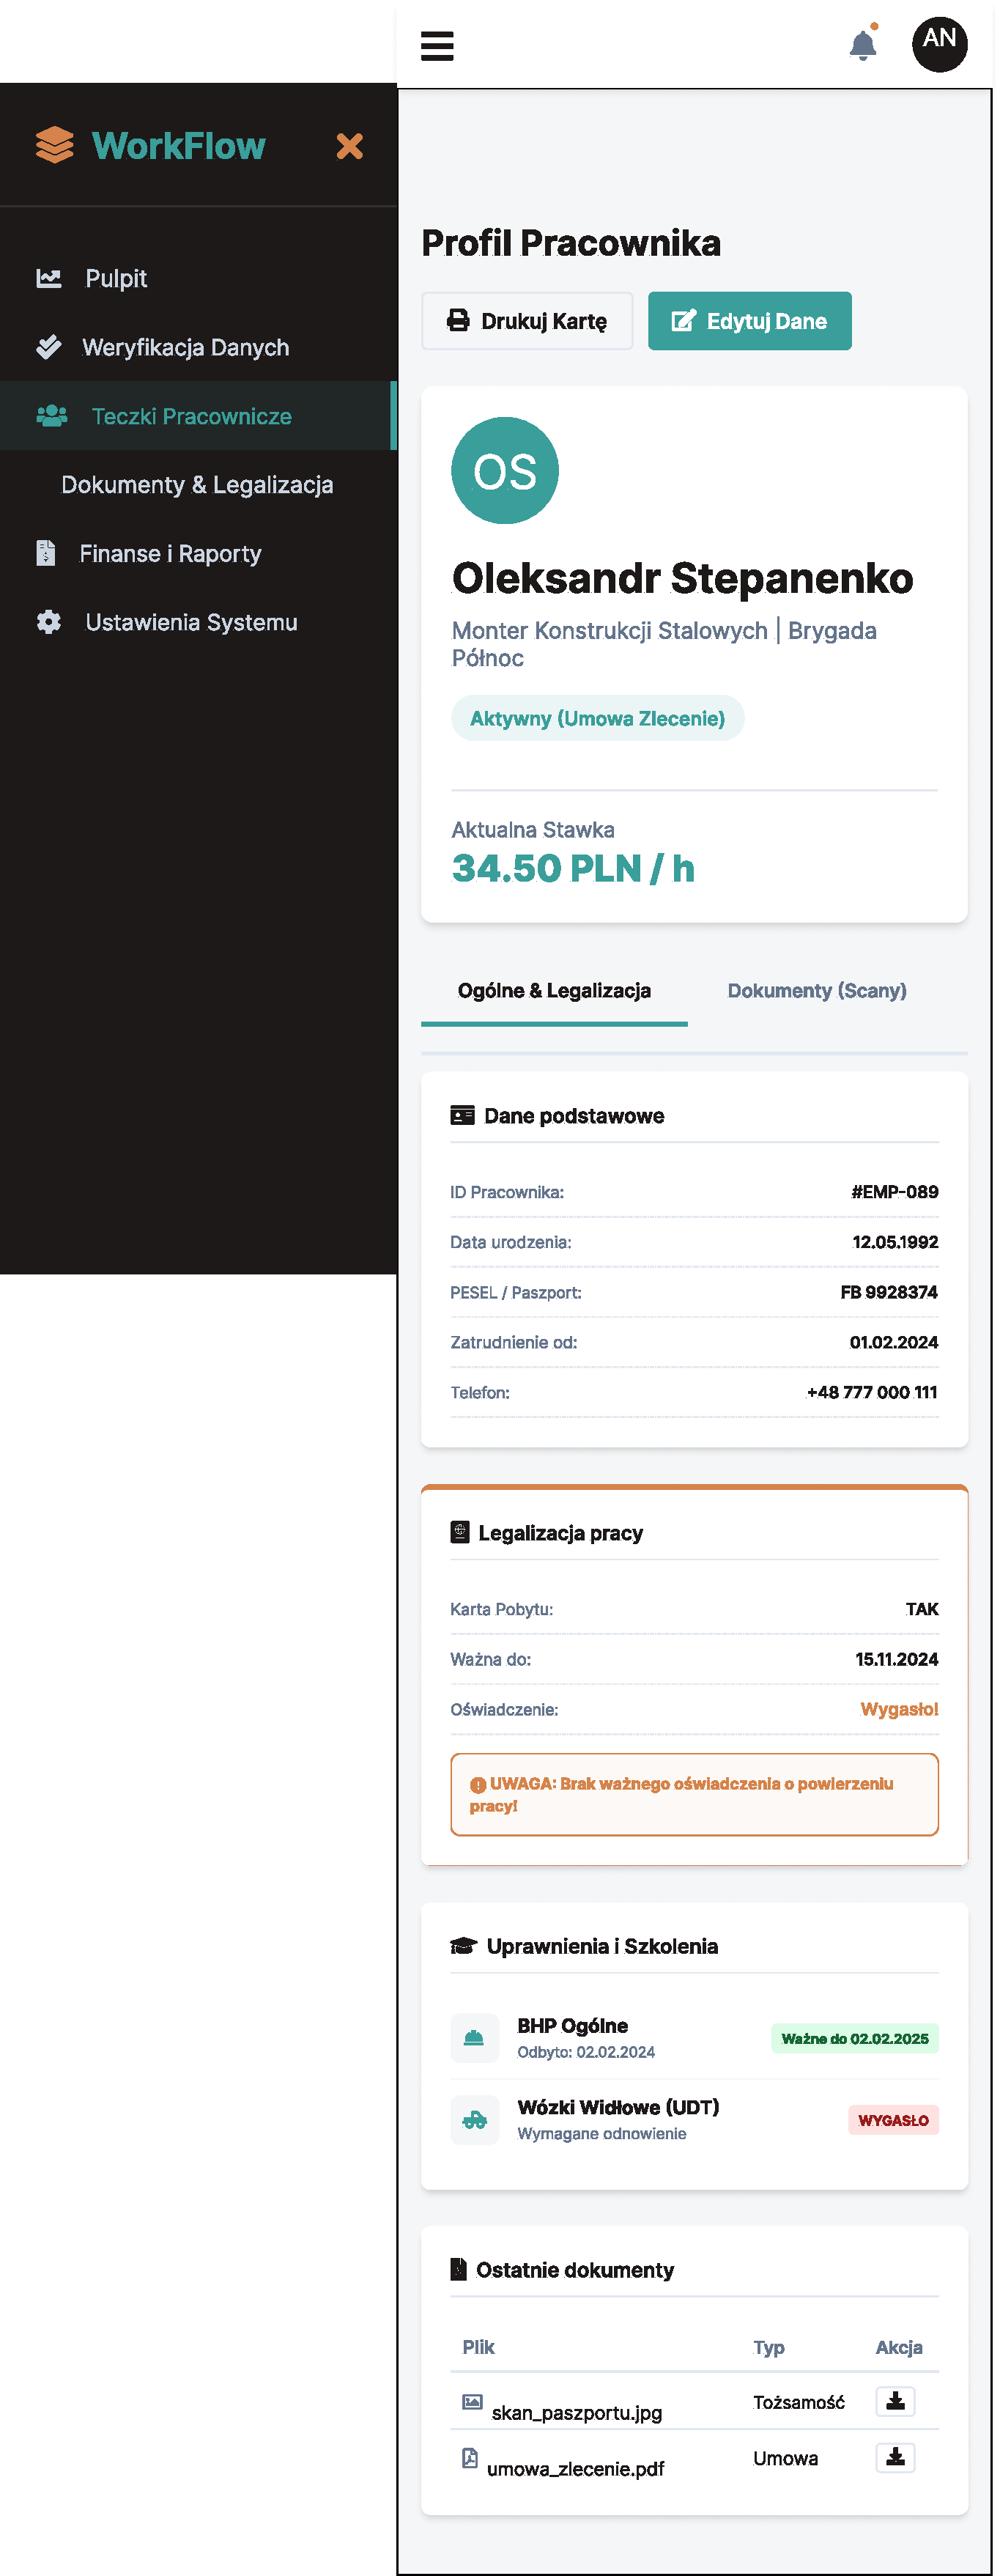
\includegraphics[width=0.35\textwidth]{rys/390w_panel.pdf}
    \caption{Widok mobilny -- profil pracownika}
    \label{fig:figma_profile_mobile}
\end{figure}

\textbf{Zakres danych prezentowanych w profilu pracownika:}
\begin{itemize}
    \item dane podstawowe, takie jak imię, nazwisko, PESEL, e-mail, rola i status aktywności,
    \item przypisanie do zakładu,
    \item identyfikator karty RFID,
    \item umowy pracownika,
    \item certyfikaty, badania i szkolenia,
    \item dokumenty powiązane z pracownikiem,
    \item nieobecności,
    \item przypisania do projektów,
    \item wpisy czasu pracy.
\end{itemize}

Profil pracownika pełni funkcję centralnego widoku kadrowego. Dzięki temu użytkownik nie musi szukać danych pracownika w wielu niezależnych miejscach. Powiązane informacje są prezentowane w jednym kontekście, co ułatwia obsługę danych kadrowych i organizacyjnych.

\subsection{Widoki tabelaryczne}

Znaczna część interfejsu systemu opiera się na widokach tabelarycznych. Dotyczy to między innymi listy pracowników, zakładów, projektów, certyfikatów, czasu pracy oraz widoków rozliczeniowych.

Widoki tabelaryczne powinny umożliwiać:
\begin{itemize}
    \item szybkie przeglądanie większej liczby rekordów,
    \item wyszukiwanie danych,
    \item filtrowanie według wybranych kryteriów,
    \item przejście do szczegółów rekordu,
    \item prezentację statusów w czytelnej formie,
    \item zachowanie spójnego układu kolumn i akcji.
\end{itemize}

W przypadku listy pracowników szczególne znaczenie mają filtry po imieniu, nazwisku, adresie e-mail, numerze PESEL, roli oraz statusie. Dla certyfikatów istotne są natomiast typ, nazwa, data ważności oraz liczba dni pozostałych do wygaśnięcia.

\subsection{Formularze}

System wykorzystuje formularze do dodawania i edycji danych. Formularze występują między innymi w modułach pracowników, zakładów, projektów, umów, certyfikatów i nieobecności.

Podczas projektowania formularzy przyjęto, że:
\begin{itemize}
    \item pola powinny być opisane w sposób jednoznaczny,
    \item dane wymagane powinny być walidowane przed zapisem,
    \item błędy powinny być prezentowane użytkownikowi w czytelny sposób,
    \item formularze powinny być możliwie krótkie i dostosowane do kontekstu,
    \item po zapisie danych użytkownik powinien otrzymać informację o rezultacie operacji.
\end{itemize}

Przykładem takiego formularza jest edycja danych pracownika, gdzie użytkownik może zaktualizować dane osobowe, adres e-mail, numer PESEL, identyfikator karty RFID, rolę oraz status aktywności.

\subsection{Tryb jasny i ciemny}

W systemie przewidziano obsługę trybu jasnego i ciemnego. Wymagało to ujednolicenia kolorów tła, tekstu, obramowań, pól formularzy oraz elementów tabelarycznych.

Obsługa dwóch motywów ma znaczenie praktyczne, ponieważ aplikacja może być używana w różnych warunkach oświetleniowych. Dodatkowo wymusza ona bardziej konsekwentne stosowanie tokenów kolorystycznych zamiast sztywnych kolorów przypisanych wyłącznie do jednego motywu.

\subsection{Znaczenie makiet dla implementacji}

Makiety stanowiły punkt wyjścia do określenia sposobu prezentacji danych oraz układu najważniejszych widoków. W trakcie implementacji część założeń została zmodyfikowana, aby lepiej dopasować interfejs do aktualnego modelu danych i dostępnych modułów.

Najważniejsze decyzje wynikające z pracy nad interfejsem to:
\begin{itemize}
    \item wykorzystanie bocznej nawigacji jako głównego sposobu poruszania się po aplikacji,
    \item centralne znaczenie profilu pracownika,
    \item prezentowanie powiązanych danych w sekcjach,
    \item stosowanie tabel dla list rekordów,
    \item oddzielenie widoków operacyjnych od widoków administracyjnych,
    \item zachowanie spójności wyglądu pomiędzy trybem jasnym i ciemnym.
\end{itemize}

W rezultacie interfejs użytkownika został podporządkowany strukturze danych oraz najważniejszym procesom systemu.
% ================= SEKCJA 8 =================
\section{Model danych i diagram ERD}

Model danych stanowi podstawę działania systemu \texttt{WorkFlow}. To w bazie danych przechowywane są informacje o pracownikach, zakładach, projektach, umowach, certyfikatach, dokumentach, nieobecnościach, zdarzeniach RCP, wpisach czasu pracy oraz eksportach rozliczeniowych. Poprawne zaprojektowanie relacji pomiędzy tymi danymi ma bezpośredni wpływ na spójność systemu oraz możliwość dalszego rozwoju aplikacji.

W projekcie wykorzystano relacyjną bazę danych PostgreSQL oraz narzędzie Prisma ORM. Schemat bazy został zdefiniowany w pliku \texttt{schema.prisma}, natomiast graficzna reprezentacja modelu została przygotowana w postaci diagramu ERD.

\begin{figure}[H]
    \centering
    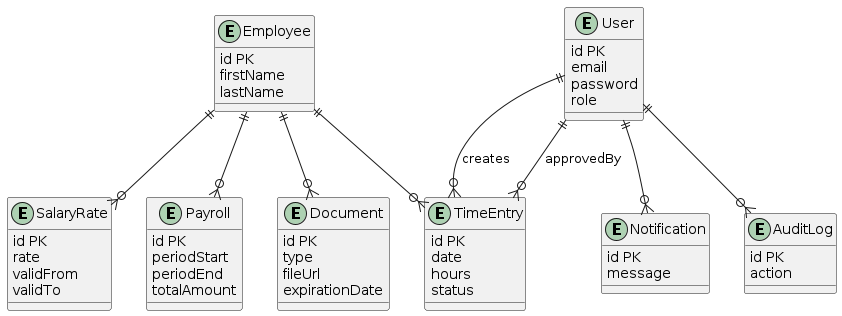
\includegraphics[width=\textwidth, height=0.8\textheight, keepaspectratio]{rys/erd.png} 
    \caption{Logiczny model danych systemu \texttt{WorkFlow}}
    \label{fig:erd_diagram}
\end{figure}

\subsection{Założenia modelu danych}

Podczas projektowania modelu danych przyjęto kilka podstawowych założeń. Pierwszym z nich było zastosowanie identyfikatorów typu \texttt{UUID} jako kluczy głównych. Rozwiązanie to pozwala na jednoznaczne identyfikowanie rekordów i jest wygodne w systemach, które mogą być rozwijane o dodatkowe integracje lub wiele środowisk uruchomieniowych.

Drugim założeniem było rozdzielenie danych źródłowych od danych przetworzonych. Najlepiej widać to w module czasu pracy. Tabela \texttt{TimeEvent} przechowuje surowe zdarzenia pochodzące z czytników RCP, natomiast tabela \texttt{TimeEntry} przechowuje przetworzone wpisy czasu pracy, które mogą być dalej weryfikowane i wykorzystywane w rozliczeniach.

Trzecim założeniem było powiązanie danych z zakładami. Pracownicy, projekty i czytniki RCP są przypisane do zakładu, co pozwala ograniczać zakres widocznych danych w zależności od uprawnień użytkownika.

Model danych został ograniczony do modułów obecnych w aktualnym zakresie projektu. Z tego względu w dokumentacji i diagramie nie uwzględniono modułu sprzętu, ponieważ został on wyłączony z zakresu realizowanej aplikacji.

\subsection{Podział modelu na obszary}

Model danych można podzielić na pięć głównych obszarów logicznych:
\begin{itemize}
    \item \textbf{Struktura organizacyjna} -- obejmuje zakłady, pracowników, dostęp do zakładów, projekty oraz przypisania pracowników do projektów.
    \item \textbf{Rejestracja czasu pracy} -- obejmuje czytniki RCP, surowe zdarzenia wejścia i wyjścia oraz przetworzone wpisy czasu pracy.
    \item \textbf{Kadry i dokumentacja} -- obejmuje umowy, dokumenty, certyfikaty, słownik certyfikatów oraz nieobecności.
    \item \textbf{Rozliczenia} -- obejmuje eksporty payroll oraz powiązanie zatwierdzonych wpisów czasu pracy z paczką rozliczeniową.
    \item \textbf{Audyt} -- obejmuje rejestrowanie wybranych operacji wykonywanych na danych systemu.
\end{itemize}

Taki podział ułatwia analizę modelu oraz pokazuje, które tabele pełnią funkcję centralną, a które są tabelami pomocniczymi lub relacyjnymi.

\subsection{Słownik głównych encji}

W tabeli \ref{tab:main_entities} przedstawiono najważniejsze encje występujące w modelu danych systemu \texttt{WorkFlow}.

\begin{table}[H]
\centering
\renewcommand{\arraystretch}{1.25}
\begin{tabular}{|p{0.24\textwidth}|p{0.68\textwidth}|}
\hline
\textbf{Encja} & \textbf{Znaczenie w systemie} \\ \hline
\texttt{Facility} & Zakład lub jednostka organizacyjna. Do zakładu przypisywani są pracownicy, projekty oraz czytniki RCP. \\ \hline
\texttt{Employee} & Centralna tabela osób. Przechowuje dane pracownika oraz dane konta użytkownika, takie jak e-mail, rola, status aktywności i identyfikator karty RFID. \\ \hline
\texttt{EmployeeFacilityAccess} & Tabela określająca, do których zakładów użytkownik posiada dostęp. Umożliwia obsługę wielu zakładów przez jednego użytkownika. \\ \hline
\texttt{Project} & Projekt, budowa lub miejsce pracy. Jest przypisany do zakładu i może posiadać przypisanych pracowników oraz czytniki RCP. \\ \hline
\texttt{EmployeeAssignment} & Historia przypisań pracowników do projektów. Pozwala określić, kto, od kiedy i do jakiego projektu został przypisany. \\ \hline
\texttt{Reader} & Czytnik RCP. Jest powiązany z zakładem oraz projektem i służy do rejestrowania zdarzeń czasu pracy. \\ \hline
\texttt{TimeEvent} & Surowe zdarzenie z czytnika RCP. Przechowuje informację o pracowniku, czytniku, typie zdarzenia oraz czasie odbicia. \\ \hline
\texttt{TimeEntry} & Przetworzony wpis czasu pracy utworzony na podstawie zdarzeń \texttt{IN} i \texttt{OUT}. Zawiera czas rozpoczęcia, zakończenia, liczbę godzin i status. \\ \hline
\texttt{Contract} & Umowa pracownika. Przechowuje typ umowy, wynagrodzenie, daty obowiązywania oraz informację, czy umowa jest aktualna. \\ \hline
\texttt{CertificationDictionary} & Słownik typów certyfikatów, szkoleń, badań i uprawnień. \\ \hline
\texttt{EmployeeCertification} & Konkretny certyfikat przypisany do pracownika, wraz z datą wydania i datą ważności. \\ \hline
\texttt{Absence} & Nieobecność pracownika, na przykład urlop, L4, nieobecność nieusprawiedliwiona lub specjalna. \\ \hline
\texttt{Document} & Metadane dokumentu pracownika. Plik przechowywany jest w MinIO, a baza przechowuje jego nazwę, lokalizację i powiązania. \\ \hline
\texttt{PayrollExport} & Eksport rozliczeniowy obejmujący zatwierdzone wpisy czasu pracy dla danego okresu. \\ \hline
\texttt{AuditLog} & Rejestr wybranych operacji wykonanych w systemie. Przechowuje akcję, encję, identyfikator rekordu oraz wartości przed i po zmianie. \\ \hline
\end{tabular}
\caption{Główne encje modelu danych systemu \texttt{WorkFlow}}
\label{tab:main_entities}
\end{table}

\subsection{Struktura organizacyjna}

Podstawą modelu organizacyjnego jest tabela \texttt{Facility}. Reprezentuje ona zakład lub jednostkę organizacyjną. Z zakładem powiązani są pracownicy, projekty oraz czytniki RCP. Dzięki temu dane można grupować według lokalizacji lub oddziałów.

Tabela \texttt{Employee} pełni podwójną rolę. Z jednej strony przechowuje dane pracownika, takie jak imię, nazwisko, PESEL, status aktywności i identyfikator karty RFID. Z drugiej strony zawiera pola potrzebne do logowania, takie jak adres e-mail, hash hasła, rola systemowa oraz flaga określająca, czy logowanie jest włączone.

Dostęp użytkowników do zakładów został opisany w tabeli \texttt{EmployeeFacilityAccess}. Dzięki temu użytkownik może posiadać dostęp do więcej niż jednego zakładu. Jest to istotne szczególnie dla administratora, HR lub księgowości, którzy mogą obsługiwać dane wielu jednostek.

Relacja pomiędzy pracownikiem a projektem została zrealizowana przez tabelę \texttt{EmployeeAssignment}. Tabela ta umożliwia przechowywanie historii przypisań, a nie tylko aktualnego stanu. Dzięki temu można określić, w jakim okresie pracownik był związany z danym projektem.

\subsection{Rejestracja czasu pracy}

Moduł czasu pracy składa się z trzech głównych tabel: \texttt{Reader}, \texttt{TimeEvent} oraz \texttt{TimeEntry}.

Tabela \texttt{Reader} przechowuje informacje o czytniku RCP. Czytnik posiada numer seryjny, nazwę lokalizacji oraz powiązanie z zakładem i projektem. Oznacza to, że zdarzenie odbicia karty na czytniku można powiązać nie tylko z pracownikiem, ale również z miejscem pracy.

Tabela \texttt{TimeEvent} przechowuje surowe zdarzenia z czytników. Każde zdarzenie zawiera pracownika, czytnik, typ zdarzenia oraz czas zdarzenia. Typ zdarzenia jest ograniczony do dwóch wartości: \texttt{IN} oraz \texttt{OUT}.

Tabela \texttt{TimeEntry} przechowuje dane przetworzone. Wpis czasu pracy powstaje na podstawie pary zdarzeń wejścia i wyjścia. Zawiera on czas rozpoczęcia, czas zakończenia, wyliczoną liczbę godzin, projekt oraz status wpisu.

\begin{table}[H]
\centering
\renewcommand{\arraystretch}{1.25}
\begin{tabular}{|p{0.24\textwidth}|p{0.20\textwidth}|p{0.44\textwidth}|}
\hline
\textbf{Pole} & \textbf{Typ} & \textbf{Opis} \\ \hline
\texttt{id} & UUID & Klucz główny wpisu czasu pracy. \\ \hline
\texttt{payrollExportId} & UUID, opcjonalny & Powiązanie z eksportem rozliczeniowym, jeżeli wpis został już ujęty w paczce payroll. \\ \hline
\texttt{employeeId} & UUID & Pracownik, którego dotyczy wpis czasu pracy. \\ \hline
\texttt{projectId} & UUID & Projekt, na którym pracownik wykonywał pracę. \\ \hline
\texttt{startTime} & timestamp & Czas rozpoczęcia pracy. \\ \hline
\texttt{endTime} & timestamp & Czas zakończenia pracy. \\ \hline
\texttt{calculatedHours} & numeric(5,2) & Wyliczona liczba przepracowanych godzin. \\ \hline
\texttt{status} & \texttt{TimeEntryStatus} & Status wpisu czasu pracy: \texttt{PENDING}, \texttt{APPROVED} lub \texttt{REJECTED}. \\ \hline
\texttt{createdAt} & timestamp & Data utworzenia wpisu. \\ \hline
\end{tabular}
\caption{Struktura tabeli \texttt{TimeEntry}}
\label{tab:timeentry_struct}
\end{table}

Rozdzielenie \texttt{TimeEvent} i \texttt{TimeEntry} jest ważne projektowo. Pozwala zachować pierwotne dane z urządzenia, a jednocześnie tworzyć dane robocze, które mogą być zatwierdzane, odrzucane lub eksportowane do rozliczeń.

\subsection{Kadry i dokumentacja}

Dane kadrowe zostały rozbite na kilka tabel, aby uniknąć przechowywania wszystkich informacji bezpośrednio w tabeli pracownika. Takie podejście poprawia czytelność modelu i umożliwia przechowywanie historii.

Tabela \texttt{Contract} przechowuje umowy pracownika. Każda umowa posiada typ, kwotę wynagrodzenia, datę rozpoczęcia, opcjonalną datę zakończenia oraz informację, czy jest aktualna. Pozwala to przechowywać zarówno bieżące, jak i historyczne warunki zatrudnienia.

Tabele \texttt{CertificationDictionary} i \texttt{EmployeeCertification} obsługują certyfikaty, badania i szkolenia. Pierwsza tabela definiuje słownik możliwych certyfikatów, natomiast druga przechowuje konkretne certyfikaty przypisane do pracowników. Dzięki temu można kontrolować daty ważności dokumentów.

Tabela \texttt{Absence} przechowuje nieobecności pracowników. Zawiera typ nieobecności, zakres dat, status zatwierdzenia oraz opcjonalne powiązanie z dokumentem.

Tabela \texttt{Document} przechowuje metadane dokumentów. Sam plik nie jest zapisywany bezpośrednio w bazie danych. W bazie przechowywana jest nazwa pliku, adres lub ścieżka do pliku oraz powiązanie z pracownikiem, umową lub certyfikatem.

\subsection{Rozliczenia}

Tabela \texttt{PayrollExport} reprezentuje paczkę danych rozliczeniowych dla danego miesiąca i roku. Przechowuje informację o użytkowniku, który wygenerował eksport, liczbie pracowników objętych eksportem oraz opcjonalnej ścieżce do pliku eksportu.

Z tabelą \texttt{PayrollExport} powiązana jest tabela \texttt{TimeEntry}. Jeżeli pole \texttt{payrollExportId} w tabeli \texttt{TimeEntry} jest wypełnione, oznacza to, że dany wpis czasu pracy został ujęty w konkretnej paczce rozliczeniowej. Takie rozwiązanie ogranicza ryzyko ponownego rozliczenia tych samych godzin.

\subsection{Audit log}

Tabela \texttt{AuditLog} została przewidziana do rejestrowania wybranych operacji wykonywanych na danych systemu. Każdy wpis audytowy zawiera użytkownika wykonującego operację, nazwę akcji, nazwę encji, identyfikator rekordu oraz opcjonalnie wartości przed zmianą i po zmianie.

Zastosowanie pól typu \texttt{Json} pozwala przechowywać zmiany w elastycznej formie, bez konieczności tworzenia osobnych tabel dla każdego rodzaju operacji. Mechanizm ten jest szczególnie przydatny przy analizie zmian dotyczących danych kadrowych, umów lub wpisów czasu pracy.

\subsection{Typy wyliczeniowe}

W modelu danych zastosowano kilka typów wyliczeniowych, które ograniczają możliwe wartości wybranych pól. Dzięki temu baza danych nie przyjmuje przypadkowych wartości tekstowych, a aplikacja może opierać się na stałym zbiorze statusów i kategorii.

Najważniejsze typy wyliczeniowe to:
\begin{itemize}
    \item \texttt{UserRole} -- role użytkowników: \texttt{ADMIN}, \texttt{HR}, \texttt{OFFICE}, \texttt{FOREMAN}, \texttt{ACCOUNTING}, \texttt{WORKER},
    \item \texttt{ProjectStatus} -- statusy projektów: \texttt{PLANNED}, \texttt{ACTIVE}, \texttt{COMPLETED}, \texttt{SUSPENDED},
    \item \texttt{TimeEventAction} -- typy zdarzeń RCP: \texttt{IN}, \texttt{OUT},
    \item \texttt{TimeEntryStatus} -- statusy wpisów czasu pracy: \texttt{PENDING}, \texttt{APPROVED}, \texttt{REJECTED},
    \item \texttt{ContractType} -- typy umów: \texttt{UOP}, \texttt{UZ}, \texttt{UD}, \texttt{B2B},
    \item \texttt{CertificationType} -- typy certyfikatów: \texttt{BHP}, \texttt{MEDICAL}, \texttt{UDT}, \texttt{OTHER},
    \item \texttt{AbsenceType} -- typy nieobecności: \texttt{HOLIDAY}, \texttt{SICK\_LEAVE}, \texttt{UNEXCUSED}, \texttt{SPECIAL}.
\end{itemize}

\subsection{Implementacja fizyczna bazy danych}

Fizyczna struktura bazy danych jest generowana na podstawie modeli Prisma. Przykładowa definicja tabeli \texttt{TimeEntry} w schemacie Prisma wygląda następująco:

\begin{lstlisting}[language=SQL, caption=Fragment modelu TimeEntry w schemacie Prisma]
model TimeEntry {
  id              String          @id @default(dbgenerated("gen_random_uuid()")) @db.Uuid
  payrollExportId String?         @db.Uuid
  employeeId      String          @db.Uuid
  projectId       String          @db.Uuid
  startTime       DateTime        @db.Timestamp(6)
  endTime         DateTime        @db.Timestamp(6)
  calculatedHours Decimal         @db.Decimal(5, 2)
  status          TimeEntryStatus @default(PENDING)
  createdAt       DateTime        @default(now()) @db.Timestamp(6)

  payrollExport   PayrollExport?  @relation(fields: [payrollExportId], references: [id])
  employee        Employee        @relation(fields: [employeeId], references: [id])
  project         Project         @relation(fields: [projectId], references: [id])
}
\end{lstlisting}

W praktyce struktura bazy może zostać zsynchronizowana z modelem Prisma za pomocą polecenia:

\begin{lstlisting}[language=bash, caption=Synchronizacja bazy danych ze schematem Prisma]
docker compose -f docker-compose.prod.yml --env-file .env exec backend npx prisma db push --config prisma.config.ts
\end{lstlisting}

Takie podejście pozwala utrzymać jedno źródło prawdy dla struktury bazy danych w kodzie projektu.

\subsection{Strategia dostępu do danych}

Backend komunikuje się z bazą danych za pomocą Prisma ORM. Prisma odpowiada za mapowanie modeli aplikacji na tabele bazy danych, wykonywanie zapytań oraz obsługę relacji pomiędzy encjami.

W projekcie większość operacji może być realizowana przez standardowe zapytania ORM. Dotyczy to między innymi dodawania pracowników, edycji danych, pobierania list, tworzenia umów, certyfikatów, nieobecności oraz wpisów czasu pracy.

W przypadku bardziej złożonych raportów lub eksportów możliwe jest wykorzystanie zapytań agregujących. Aktualna wersja projektu skupia się jednak przede wszystkim na czytelnym modelu relacyjnym i poprawnym powiązaniu danych, a nie na zaawansowanej analityce SQL.

\subsection{Znaczenie modelu danych dla systemu}

Model danych systemu \texttt{WorkFlow} został zaprojektowany tak, aby odwzorować podstawowe zależności występujące w procesach kadrowych i ewidencji czasu pracy. Najważniejszą encją jest pracownik, który łączy się z większością pozostałych obszarów systemu: zakładami, projektami, dokumentami, certyfikatami, umowami, nieobecnościami i czasem pracy.

Dzięki relacyjnemu modelowi danych system może zachować spójność pomiędzy modułami. Przykładowo wpis czasu pracy nie istnieje samodzielnie, lecz jest powiązany z pracownikiem i projektem. Dokument nie jest anonimowym plikiem, lecz posiada właściciela i może być powiązany z umową lub certyfikatem. Certyfikat nie jest tylko tekstową informacją, ale wynika ze słownika i posiada datę ważności.

Takie ustrukturyzowanie danych umożliwia dalszy rozwój systemu, między innymi o dodatkowe raporty, powiadomienia, integracje księgowe lub bardziej rozbudowane mechanizmy kontroli dostępu.
% ================= SEKCJA 9 =================
\section{Wykorzystanie narzędzi AI w procesie realizacji projektu}

W trakcie realizacji projektu \texttt{WorkFlow} autor korzystał z narzędzi opartych na sztucznej inteligencji jako wsparcia w analizie problemów, porządkowaniu zadań, redagowaniu dokumentacji oraz weryfikacji wybranych rozwiązań technicznych. Wykorzystywane były przede wszystkim narzędzia ChatGPT oraz Gemini, przy czym ChatGPT był używany częściej ze względu na lepsze dopasowanie odpowiedzi do kontekstu projektu i możliwość prowadzenia dłuższej, spójnej pracy nad kolejnymi etapami systemu.

Narzędzia AI nie zastępowały samodzielnej realizacji projektu. Pełniły funkcję konsultacyjną, podobną do korzystania z dokumentacji technicznej, wyszukiwarki, forów programistycznych lub narzędzi wspierających analizę kodu. Ostateczne decyzje projektowe, implementacyjne i redakcyjne były podejmowane przez autora projektu, a zaproponowane rozwiązania były każdorazowo weryfikowane w praktyce.

\subsection{Zakres wykorzystania narzędzi AI}

Narzędzia AI były wykorzystywane głównie w tych obszarach, w których przyspieszały analizę lub pomagały uporządkować pracę. Dotyczyło to zarówno części programistycznej, jak i dokumentacyjnej projektu.

Najważniejsze zastosowania obejmowały:
\begin{itemize}
    \item analizę błędów pojawiających się podczas pracy nad frontendem i backendem,
    \item interpretację komunikatów TypeScript, ESLint, Prisma, Docker oraz Node.js,
    \item porządkowanie kolejności zadań wykonywanych w projekcie,
    \item przygotowywanie propozycji komend testowych i diagnostycznych,
    \item analizę problemów z uruchomieniem aplikacji w kontenerach Docker,
    \item wsparcie przy konfiguracji środowiska produkcyjnego,
    \item pomoc w przygotowaniu danych demonstracyjnych,
    \item redagowanie i aktualizację dokumentacji technicznej,
    \item upraszczanie zbyt rozbudowanych lub nieprecyzyjnych opisów.
\end{itemize}

Szczególnie istotne było wykorzystanie AI jako narzędzia do bieżącej analizy problemów. W przypadku pojawienia się błędu autor mógł przedstawić komunikat z terminala lub fragment kodu, a następnie otrzymać propozycję przyczyny problemu oraz możliwych kroków diagnostycznych.

\subsection{Wsparcie podczas implementacji}

Podczas implementacji systemu narzędzia AI były wykorzystywane do analizy i wyjaśniania problemów technicznych. Dotyczyło to między innymi błędów kompilacji TypeScript, ostrzeżeń ESLint, problemów z działaniem formularzy, konfiguracją zmiennych środowiskowych oraz uruchomieniem aplikacji w Dockerze.

Przykładowe obszary, w których AI wspierało pracę implementacyjną, to:
\begin{itemize}
    \item analiza błędów związanych z typami danych w TypeScript,
    \item poprawianie problemów wykrywanych przez ESLint,
    \item diagnozowanie problemów z logowaniem użytkownika,
    \item analiza konfiguracji frontendowego adresu API,
    \item pomoc przy konfiguracji Dockerfile dla frontendu i backendu,
    \item analiza błędów uruchamiania aplikacji w kontenerach,
    \item wsparcie przy pracy z Prisma i inicjalizacji bazy danych,
    \item przygotowanie oraz weryfikacja seedów bazy danych.
\end{itemize}

W praktyce AI nie było traktowane jako źródło gotowych, bezwarunkowo poprawnych rozwiązań. Każda propozycja wymagała sprawdzenia w kodzie, uruchomienia aplikacji oraz oceny, czy pasuje do aktualnej struktury projektu. W wielu przypadkach wygenerowane sugestie wymagały modyfikacji, uproszczenia albo dostosowania do istniejących plików i konwencji.

\subsection{Wsparcie przy konfiguracji środowiska}

Istotnym elementem projektu było przygotowanie środowiska uruchomieniowego opartego na Docker Compose. W tym obszarze narzędzia AI pomagały w analizie zależności pomiędzy kontenerami, sposobie przekazywania zmiennych środowiskowych oraz diagnozowaniu błędów wynikających z różnic pomiędzy środowiskiem lokalnym a kontenerowym.

AI wspierało między innymi analizę problemów związanych z:
\begin{itemize}
    \item brakiem zbudowanych plików aplikacji w katalogu \texttt{dist},
    \item błędną ścieżką startową backendu,
    \item brakiem wymaganych zmiennych środowiskowych w kontenerze,
    \item konfiguracją połączenia Prisma z bazą PostgreSQL,
    \item przekierowaniem ruchu przez Nginx,
    \item różnicą pomiędzy adresem API widocznym dla przeglądarki a adresem API widocznym wewnątrz sieci Docker.
\end{itemize}

W tym zakresie AI pełniło rolę pomocniczą przy interpretacji logów i wskazywaniu kolejnych komend diagnostycznych. Ostateczna weryfikacja odbywała się poprzez uruchomienie kontenerów, analizę logów, testowanie endpointów za pomocą \texttt{curl} oraz sprawdzenie działania aplikacji w przeglądarce.

\subsection{Wsparcie przy danych demonstracyjnych}

Narzędzia AI zostały również wykorzystane podczas przygotowywania danych demonstracyjnych. Dane te były potrzebne do prezentacji działania systemu bez konieczności ręcznego wprowadzania dużej liczby rekordów.

Wsparcie AI obejmowało:
\begin{itemize}
    \item zaplanowanie zakresu danych demonstracyjnych,
    \item przygotowanie struktury seeda prezentacyjnego,
    \item analizę błędów TypeScript w skrypcie seedującym,
    \item uporządkowanie danych testowych tak, aby obejmowały najważniejsze moduły systemu,
    \item dodanie zabezpieczenia przed przypadkowym uruchomieniem destrukcyjnego seeda.
\end{itemize}

Dzięki temu możliwe było przygotowanie danych obejmujących użytkowników, zakłady, pracowników, projekty, czytniki RCP, umowy, certyfikaty, dokumenty, nieobecności, wpisy czasu pracy oraz przykładowy eksport rozliczeniowy. Dane te zostały następnie sprawdzone w działającej aplikacji.

\subsection{Wsparcie przy dokumentacji}

Drugim ważnym obszarem wykorzystania narzędzi AI była dokumentacja projektu. W tym przypadku AI pomagało przede wszystkim w porządkowaniu treści, aktualizacji opisów do aktualnego stanu aplikacji oraz usuwaniu zbyt ogólnych lub przesadnie marketingowych sformułowań.

W dokumentacji AI wspierało:
\begin{itemize}
    \item redakcję opisu celu projektu,
    \item uporządkowanie wymagań funkcjonalnych i niefunkcyjnych,
    \item aktualizację scenariuszy użycia,
    \item opis modelu danych i diagramu ERD,
    \item opis stosu technologicznego,
    \item przygotowanie instrukcji prezentacji projektu,
    \item ujednolicenie stylu językowego dokumentacji.
\end{itemize}

Ważnym założeniem było zachowanie formalnego charakteru dokumentacji bez nadmiernego rozbudowywania opisów. Z tego powodu część propozycji była upraszczana lub odrzucana, jeżeli brzmiała zbyt marketingowo albo sugerowała funkcje, które nie zostały zaimplementowane w aktualnej wersji projektu.

\subsection{Weryfikacja odpowiedzi generowanych przez AI}

Korzystanie z narzędzi AI wymagało zachowania ostrożności. Odpowiedzi generowane przez modele językowe mogą być niepełne, nieaktualne albo niedopasowane do konkretnego projektu. Z tego względu żadna propozycja nie była traktowana jako automatycznie poprawna.

Weryfikacja odbywała się poprzez:
\begin{itemize}
    \item analizę istniejącego kodu źródłowego,
    \item uruchamianie aplikacji lokalnie,
    \item sprawdzanie logów backendu, frontendu i kontenerów,
    \item testowanie endpointów za pomocą zapytań HTTP,
    \item kontrolę działania funkcji w interfejsie użytkownika,
    \item sprawdzanie zmian w systemie kontroli wersji Git,
    \item porównywanie dokumentacji z rzeczywistym zakresem aplikacji.
\end{itemize}

Taki sposób pracy ograniczał ryzyko bezrefleksyjnego przyjęcia błędnych sugestii. AI było wykorzystywane jako narzędzie wspomagające analizę i organizację pracy, a nie jako samodzielny wykonawca projektu.

\subsection{Porównanie wykorzystanych narzędzi}

W trakcie pracy wykorzystywane były dwa narzędzia: Gemini oraz ChatGPT. Oba rozwiązania mogły wspierać analizę problemów i redakcję treści, jednak w praktyce większe znaczenie w projekcie miało narzędzie ChatGPT.

Gemini było wykorzystywane pomocniczo, głównie do porównywania propozycji odpowiedzi lub uzyskania alternatywnego spojrzenia na dany problem. ChatGPT okazał się bardziej przydatny podczas dłuższej pracy nad projektem, ponieważ lepiej utrzymywał kontekst kolejnych etapów, takich jak rozwój modułów, poprawki błędów, konfiguracja Docker oraz aktualizacja dokumentacji.

Nie oznacza to jednak, że odpowiedzi ChatGPT były przyjmowane bez weryfikacji. Narzędzie to było traktowane jako asystent konsultacyjny, którego propozycje należało sprawdzić i dostosować do rzeczywistego kodu projektu.

\subsection{Wpływ AI na przebieg pracy}

Wykorzystanie narzędzi AI wpłynęło przede wszystkim na tempo pracy i sposób organizacji zadań. Dzięki możliwości szybkiej analizy błędów i propozycji kolejnych kroków łatwiej było przechodzić przez problemy techniczne oraz utrzymywać porządek w realizowanych zadaniach.

Największe korzyści z wykorzystania AI to:
\begin{itemize}
    \item szybsza analiza błędów i komunikatów diagnostycznych,
    \item łatwiejsze planowanie kolejnych etapów pracy,
    \item możliwość szybkiego porównania kilku wariantów rozwiązania,
    \item wsparcie przy redakcji dokumentacji,
    \item większa konsekwencja w nazewnictwie i opisie modułów,
    \item pomoc w przygotowaniu komend testowych i diagnostycznych.
\end{itemize}

Jednocześnie wykorzystanie AI nie zwalniało autora z odpowiedzialności za projekt. Kod musiał zostać uruchomiony, przetestowany i dopasowany do istniejącej struktury aplikacji. Dokumentacja musiała zostać porównana z rzeczywistym zakresem systemu, aby nie opisywała funkcji, które nie są częścią projektu.

\subsection{Podsumowanie}

Narzędzia AI były istotnym wsparciem podczas realizacji projektu \texttt{WorkFlow}, szczególnie w zakresie analizy błędów, organizacji pracy i redakcji dokumentacji. Ich rola miała jednak charakter pomocniczy. Projekt, jego zakres, decyzje techniczne, testowanie oraz ostateczny kształt dokumentacji pozostawały pod kontrolą autora.

Takie wykorzystanie AI można traktować jako element współczesnego procesu pracy programistycznej. Narzędzia te pomagają szybciej analizować problemy i porządkować informacje, ale wymagają krytycznego podejścia, weryfikacji oraz świadomego dostosowania wygenerowanych sugestii do rzeczywistego projektu.

% ================= BIBLIOGRAFIA =================
\clearpage
\FloatBarrier
\addcontentsline{toc}{section}{Literatura}
\nocite{*}
\printbibliography

% ================= SPIS RYSUNKÓW =================
\clearpage
\FloatBarrier
\addcontentsline{toc}{section}{Spis rysunków}
\listoffigures
\thispagestyle{fancy}

% ================= SPIS TABEL =================
\clearpage
\FloatBarrier
\addcontentsline{toc}{section}{Spis tabel}
\listoftables
\thispagestyle{fancy}

% ================= SPIS LISTINGÓW =================
\clearpage
\FloatBarrier
\renewcommand\lstlistlistingname{Spis listingów}
\addcontentsline{toc}{section}{Spis listingów}
\lstlistoflistings
\thispagestyle{fancy}

% % ================= TODO (DO USUNIĘCIA PRZED ODDANIEM) =================
% % \todos

\end{document}
